%%%%%%%%%%%%%%%%%%%%%%%%%%%%%%%%%%%%%
%% Dissreta��o de Mestrado em Engenharia El�trica
%% Copyright 2009 Fabio de Oliveira Lima.
%% Este documento � distribu�do nos termos da licen�a 
%% GNU General Public License v2.
%%%%%%%%%%%%%%%%%%%%%%%%%%%%%%%%%%%%%

\documentclass[dvips,ruledheader, tocpage=plain]{abnt}%, pagestart=firstchapter
\usepackage[latin1]{inputenc}
%\usepackage[num]{abntcite}
%\usepackage[alf]{abntcite}
\usepackage{abnt-alf}
\usepackage[dvips]{graphicx}
\usepackage[brazil]{babel}
\usepackage{srcltx}

% \usepackage{fullpage}
% \usepackage{color}
% \usepackage{graphicx}
% \usepackage{epsfig}
\usepackage{amsthm}
\usepackage{latexsym}
\usepackage{amssymb}
\usepackage{amsmath}
% \usepackage{srcltx}

% Acrescentado por mim: CyberToddy

\usepackage[T1]{fontenc}
% \usepackage[latin1]{inputenc}
% \sloppy

% example environment
% \newenvironment{example}
% {\emph{Exemplo:}}
% {\hfill $\boxtimes$\newline\newline}


% \newcommand{\zz} {\vspace {0.3cm}} 
\newcommand{\z}{\par}
\newcommand{\bsq}{\z \hfill$\blacksquare$}
\newcommand{\rr}{$^{\text{\textregistered}}$}
\newcommand{\Forall}[1]{,\quad\forall\, \mbox{\small$#1$}}


\newenvironment{solucao}
{\emph{Solu��o:}}
{\hfill $\boxtimes$\newline\newline}

\newenvironment{dem}
{\emph{Demonstra��o:}}
{\bsq}

\numberwithin{equation}{section}

% some theorem environments
\newtheorem{theorem}{Teorema}
% \newtheorem{proposition}{Dados}
% \newtheorem{claim}{Clamor}
 \newtheorem{lemma}{Lema}
% \newtheorem{corollary}{Corol\'{a}rio}


% \newtheorem{acknowledgement}[theorem]{Agradecimentos}
% \newtheorem{algorithm}[theorem]{Algoritmo}
% \newtheorem{axiom}[theorem]{Axioma}
% \newtheorem{case}[theorem]{Caso}
% \newtheorem{conclusion}[theorem]{Conclus\~{a}o}
% \newtheorem{condition}[theorem]{Conditi\c{c}\~{a}o}
% \newtheorem{conjecture}[theorem]{Conjectura}
% \newtheorem{criterion}[theorem]{Crit\'{e}rio}
\newtheorem{notation}{Notata\c{c}\~{a}o}
\newtheorem{dados}{Dados}
\newtheorem{var}{Vari�vel}[section]
% \newtheorem{problem}[theorem]{Problema}
% \newtheorem{remark}[theorem]{Observa\c{c}\~{a}o}
% \newtheorem{solution}[theorem]{Solu\c{c}\~{a}o}
% \newtheorem{summary}[theorem]{Sum\'{a}ario}

%\newenvironment{proof}[1][Proof]{\textbf{#1.} }{\ \rule{0.5em}{0.5em}}


% \newtheorem{definition}{Defini\c{c}\~{a}o} % Use this for non-trivial



% \usepackage{latexsym}
% \usepackage{psfrag}
% \usepackage[center]{caption2}

% \usepackage{lineno}	% Numera as linhas.
% \linenumbers		% Numera as linhas, a partir do in�cio.
% \pagewiselinenumbers	% Numera as linhas de cada p�gina (Eu prefiro este). 


\begin{document}
\citeoption{abnt-show-options=no}

%\DeclareGraphicsRule{.eps.gz}{eps}{.eps.bb}{`gunzip -c #1}


% %% Capa
%% Copyright 2009 Marcelo de Oliveira Lima.
%% Este documento � distribu�do nos termos da licen�a 
%% GNU General Public License v2.

% Usando o comando \capa


\instituicao{Programa de P�s-Gradua��o em Engenharia El�trica \par 
Centro Tecnol�gico \par 
Universidade Federal do Esp�rito Santo}


\titulo{METODOLOGIA PARA O PROJETO COMPLETO DE REDES �PTICAS COM TOPOLOGIA EM HIERARQUIA}

\autor{Marcelo de Oliveira Lima}



\local{Vit�ria -- ES}

\data{\today}

\capa

% ou...
% fazendo a mao
%
% \begin{titlepage}
%
%   ... codigo da folha de rosto
%  
% \end{titlepage}


%%%%%%%%%%%%%%%%%%%%%%%%%%%%%%%%%%%%%
%%   Folha de rosto
%% Copyright 2009 Fabio de Oliveira Lima.
%% Este documento � distribu�do nos termos da licen�a 
%% GNU General Public License v2.
%%%%%%%%%%%%%%%%%%%%%%%%%%%%%%%%%%%%%

% Usando o comando \folhaderosto

\titulo{UM MODELO EFICIENTE PARA O PROJETO COMPLETO DE REDES �PTICAS}

\autor{Fabio de Oliveira Lima}

 \begin{center}
 Copyright 2009 Fabio de Oliveira Lima.\\ Este documento � distribu�do nos termos da licen�a \textbf{GNU} \textit{General Public License v2}.
 \end{center}

\orientador{Prof. Dr. Elias Silva de Oliveira}
% ou \orientador[Orientadora:\\]{Minha orientadora}

\coorientador{Marcelo Eduardo Vieira Segatto}
% ou \coorientador[Co-orientadora:\\]{Minha co-orientadora}

\comentario{Disserta��o a ser apresentada � Coordena��o do Mestrado em Engenharia El�trica
 da Universidade Federal do Esp�rito Santo para a obten��o do t�tulo de Mestre em Engenharia El�trica.}


\instituicao{Programa de P�s-Gradua��o em Engenharia El�trica \par 
	Centro de Tecnologia \par 
	Universidade Federal do Esp�rito Santo}

\local{Vit�ria -- ES}

\data{\today}

\folhaderosto


% ou...
% fazendo a mao
%
% \begin{titlepage}
%
%   ... codigo da folha de rosto
%  
% \end{titlepage}


% 
 \begin{center}
 Copyright 2009 Fabio de Oliveira Lima.\\ Este documento � distribu�do nos termos da licen�a \textbf{GNU} \textit{General Public License v2}.
 \end{center}


% %%%%%%%%%%%%%%%%%%%%%%%%%%%%%%%%%%%%%
%% Folha de Aprova��o
%% Copyright 2009 Marcelo de Oliveira Lima.
%% Este documento � distribu�do nos termos da licen�a 
%% GNU General Public License v2.
%%%%%%%%%%%%%%%%%%%%%%%%%%%%%%%%%%%%%


\begin{folhadeaprovacao}

\begin{center}
\begin{large}

MARCELO DE OLIVEIRA LIMA

\bigskip
\bigskip

\textbf{PROJETO COMPLETO DE REDES �PTICAS COM TOPOLOGIA EM HIERARQUIA}

\bigskip

\end{large}
\end{center}

Disserta��o submetida ao programa de P�s-Gradua��o em Engenharia El�trica do Centro Tecnol�gico da Universidade Federal do Esp�rito Santo, como requisito
parcial para a obten��o do Grau de Mestre em Engenharia El�trica.

\begin{flushright}
Aprovada em 26 de julho de 2010.
\end{flushright}

\begin{center}
COMISS�O EXAMINADORA
\end{center}

\setlength{\ABNTsignthickness}{0.4pt}
\setlength{\ABNTsignwidth}{10cm}
\setlength{\ABNTsignskip}{2cm}

\assinatura{Dr. Marcelo Eduardo Vieira Segatto \\ Departamento de Engenharia El�trica - UFES \\ Orientador}

\assinatura{Dra. Rosane Bodart Soares \\ Departamento de Engenharia El�trica - UFES \\ Examinador Interno}

\assinatura{Dr. Renato Tannure Rotta Almeida \\ Instituto Federal de Educa��o C\&T do Esp�rito Santo - IFES \\ Examinador Externo}

\assinatura{Dr. Carlos Renato Lisboa Franc�s \\ Faculdade de Engenharia de Computa��o - UFPA \\ Examinador Externo}

\end{folhadeaprovacao}


%%%%%%%%%%%%%%%%%%%%%%%%%%%%%%%%%%%%%
%% Epigrafe
%% Copyright 2009 Marcelo de Oliveira Lima.
%% Este documento � distribu�do nos termos da licen�a 
%% GNU General Public License v2.
%%%%%%%%%%%%%%%%%%%%%%%%%%%%%%%%%%%%%


%  Ep�grafe - � uma cita��o pertinente ao seu trabalho
%  ou que represente o seu modo de pensar. 
%  Resumindo, coloque uma frase que o(a) agrade.


\pretextualchapter{}

\vspace{17.5cm}
\begin{flushright}

\textit{``A mente que se abre a uma nova id�ia jamais voltar� ao seu tamanho original.'' \\ 
	\bfseries Albert Einstein}

\end{flushright}




%%%%%%%%%%%%%%%%%%%%%%%%%%%%%%%%%%%%%
%% Resumo
%% Copyright 2009 Marcelo de Oliveira Lima.
%% Este documento � distribu�do nos termos da licen�a 
%% GNU General Public License v2.
%%%%%%%%%%%%%%%%%%%%%%%%%%%%%%%%%%%%%

\begin{resumo}

Este trabalho apresenta uma metodologia para o projeto f�sico e l�gico de redes �pticas de comunica��o com topologia em malhas hier�rquicas. S�o
determinadas as
topologias l�gica e f�sica, al�m do roteamento e designa��o de comprimentos de onda, em fun��o da localiza��o geogr�fica dos n�s da rede. A metodologia
proposta consiste em tr�s etapas que integram uma meta-heur�stica, infer�ncia estat�stica e um modelo de programa��o linear inteira-mista. Na primeira um
algoritmo gen�tico define a estrutura hier�rquica da rede �ptica. Em seguida, um procedimento estat�stico obtem estimativas para
par�metros de interesse que ser�o usados para definir crit�rios de qualidade para o projeto, limitando as vari�veis do modelo de
programa��o matem�tica resolvido na �ltima etapa. S�o apresentados resultados de experimentos com o objetivo de validar a efici�ncia desta formula��o
quanto ao
desempenho computacional e tamb�m com rela��o � qualidade das solu��es, tendo como base de compara��o limitantes inferiores para as m�tricas
a serem otimizadas.

Palavras Chave: Redes �pticas, Otimiza��o combinat�ria.

\end{resumo}


%%%%%%%%%%%%%%%%%%%%%%%%%%%%%%%%%%%%%
%% Abstract
%% Copyright 2009 Fabio de Oliveira Lima.
%% Este documento � distribu�do nos termos da licen�a 
%% GNU General Public License v2.
%%%%%%%%%%%%%%%%%%%%%%%%%%%%%%%%%%%%%


\begin{abstract}

% Apresenta��o concisa dos pontos relevantes, dando uma visao rapida e
% clara do conte�do do trabalho.

This dissertation presents a new mixed integer linear programming model for the design of optical communication networks. This is a extensive modeling,
which includes the design of logical and physical topology, routing of traffic demands, in addition to routing and wavelength assignment. The formulation
supports multiple connections between each pair of network nodes, whether in the physical or logic topology. In its basic version, the model minimizes
installation's cost of the physical network and the  operation's cost of the network designed. However, its formulation allows  explore various metrics such
as network's congestion, which was used for comparison with literature. This work presents results of experiments in order to validate the efficiency of
this formulation with respect to quality of solutions and computational performance of previous work on the same subject. Also presented is a new way to
obtain lower bounds to congestion, with very tiny computational's cost, whose efficiency contrasts with the options found in literature.

\end{abstract}


\tableofcontents


%%%%%%%%%%%%%%%%%%%%%%%%%%%%%%%%%%%%%
%% Introdu��o
%% Copyright 2009 Marcelo de Oliveira Lima.
%% Este documento � distribu�do nos termos da licen�a 
%% GNU General Public License v2.
%%%%%%%%%%%%%%%%%%%%%%%%%%%%%%%%%%%%%


\chapter*{Introdu��o}
\label{intro}

A Multiplexa��o por Divis�o de Comprimentos de Onda (WDM), tecnologia que permite transmiss�o de v�rios sinais em diferentes comprimentos de onda
simultaneamente atrav�s de um mesmo enlace de fibra �ptica, juntamente com o Roteamento por Comprimento de Onda, realizado por n�s de rede que realizam o
roteamento dos sinais a partir do comprimento de onda dos mesmos, representam um alvo frequente de estudos nas �ltimas d�cadas.

Uma rede WDM consiste de n�s roteadores de comprimentos de onda interconectados atrav�s de enlaces ponto a ponto de fibra �ptica em uma determinada topologia.
Suas principais vantagens s�o o maior aproveitamento da largura de banda utilizada na fibra, menor custo relacionado ao processamento eletr�nico de dados nos
n�s da rede, transpar�ncia com rela��o ao protocolo de comunica��o e um eficiente tratamento/adequa��o a falhas dos componentes da rede, sejam falhas em enlaces
ou n�s. Com isso, as redes �pticas WDM com roteamento por comprimentos de onda (WRON) vem se consolidando como o padr�o de transmiss�o de dados em alta
velocidade.

Nas redes �pticas semi-transparentes \cite{ram96} parte do tr�fego a ser transmitido pela rede � transportado de maneira totalmente transparente
entre os pares de n�s que s�o interligados diretamente por caminhos �pticos. Entre os outros pares de n�s, s� � poss�vel o transporte de tr�fego atrav�s de
rotas formadas por mais de um caminho �ptico em seq��ncia. Neste segundo caso, o tr�fego deve ser processado nos n�s intermedi�rios de sua rota fonte-destino
para que  seja efetuada sua retransmiss�o pelo pr�ximo caminho �ptico. Ao se projetar redes WDM com roteamento de tr�fego por comprimento de onda, devemos
buscar uma solu��o que distribua e minimize o tr�fego alocado aos caminhos �pticos e tamb�m minimize o atraso m�dio de pacotes na rede.

Tradicionalmente o projeto de redes �pticas foi dividido em dois problemas que eram resolvidos de forma isolada \cite{ram96} \cite{murthy} \cite{mukherjee}
\cite{Karcius04}, s�o eles: Projeto da Topologia Virtual (VTD) e Roteamento e Aloca��o de Comprimentos de Onda (RWA). Nos �ltimos anos no entanto foram
apresentados na literatura abordagens integradas para os dois problemas \cite{Karcius04} \cite{Xin:03} e desta maneira o projeto de redes �pticas passou a ser
tratado de forma unificada, contemplando aspectos "f�sicos e virtuais" da rede. Os sub-problemas citados�s�o complexos e cada um deles � conhecido como
NP-Completo e a solu��o dos dois conjuntamente � ainda mais complexa. Diante disso, resolver o modelo matem�tico completo, em busca da solu��o �tima, torna-se
invi�vel. Como o objetivo � encontrar uma maneira de resolver o problema de forma integrada e com um tempo computacional�aceit�vel, o uso de de m�todos
(Meta-)Heur�sticos \cite{beas} torna-se uma boa alternativa.

\underline{\textbf{Falar de TWA, Hierarquia e teorias utilizadas...}}

A literatura recente mostra bons resultados para a estrat�gia descrita acima \cite{Karcius04} \cite{Xin:03}, ou seja, a utiliza��o de m�todos heur�sticos para
obter solu��es sub-�timas para o problema de projeto integrado de redes �pticas. Contudo, os estudos desenvolvidos at� aqui se concentraram em topologias em
malha. Para o presente trabalho de disserta��o a proposta � estender os resultados para topologias em hierarquias.

O restante deste texto est� organizado da seguinte forma: No Cap�tulo \\ref{} a seguir apresentamos.... No Cap�tulo \\ref{} � apresentada ... No Cap�tulo
\\ref{} s�o apresentados resultados computacionais obtidos....




\section{Modelagem TWA}
\label{Basic}

Nesta se��o ser� apresentada a forma b�sica do modelo TWA, come�ando pela nota��o designada aos n�s e as constantes que definem uma inst�ncia de
problema para o modelo. Em seguida ser�o definidas as vari�veis utilizadas para compor as restri��es e a fun��o objetivo do modelo, passando-se
ent�o � sua descri��o. Como os experimentos realizados neste trabalho objetivaram primariamente a compara��o da efici�ncia do TWA com resultados
previamente publicados, para efeitos de compatibilidade: o n�mero de saltos f�sicos na rede foi tomado como fun��o objetivo \cite{Karcius04}; o
n�mero de comprimentos de onda foi controlado de maneira impl�cita \cite{Zang00}; e foi considerada a restri��o de conserva��o dos comprimentos de
onda ao longo do caminho �ptico \cite{Zang00}, ou seja, n�o se admite a convers�o de comprimentos de onda na camada �ptica da rede.

\zz
\begin{notation}
Os �ndices $m,n,s,d,i,j\in \{1,..,N\}$ representam os n�s da rede, e os pares ordenados $(m,n)$, $(s,d)$ e $(i,j)$ indicam 
respectivamente liga��es f�sicas, demandas de tr�fego e liga��es l�gicas, com $m\neq n$, $s\neq d$ e $i\neq j$. O �ndice $w 
\in \{1,..,W\}$ representa os comprimentos de onda dispon�veis.
\end{notation}

% Para simplificar a nota��o das restri��es do modelo, adota-se a constante $A_s = \sum_d P_{s,d}$, que � a soma de todas 
% as demandas de tr�fego com origem em $s$, pois o tr�fego ser� agregado em rela��o � origem \cite{ram02}.

A Figura \ref{fig:Indices} ilustra os diferentes escopos dos �ndices associados aos n�s da rede, com rela��o aos enlaces f�sicos $(m,n)$, l�gicos
$(i,j)$ e demandas de tr�fego $(s,d)$. Esta nota��o segue a conven��o comumente utilizada em trabalhos anteriores \cite{mukherjee, ram02}. �
importante dizer que, como esta modelagem suporta m�ltiplas fibras e caminhos �pticos entre cada par de n�s, os pares $(m,n)$ e $(s,d)$ representam
conjuntos de poss�veis liga��es f�sicas e l�gicas, respectivamente. Esses conjuntos n�o ser�o explicitamente controlados, sendo esse um dos motivos
da efici�ncia do modelo.

\begin{figure}[hb]
\centering
% 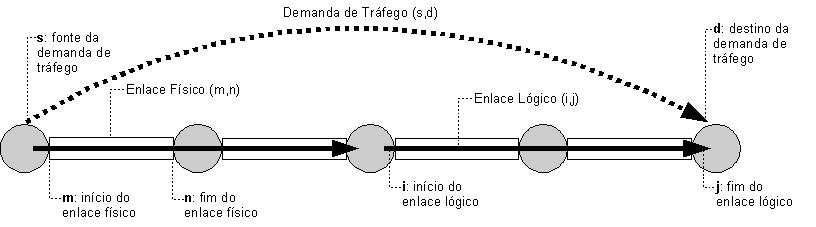
\includegraphics[bb=0 0 612 170, scale=0.7]{figs/TanA.JPG}
% TanA.JPG: 816x227 pixel, 96dpi, 21.59x6.01 cm, bb=0 0 612 170
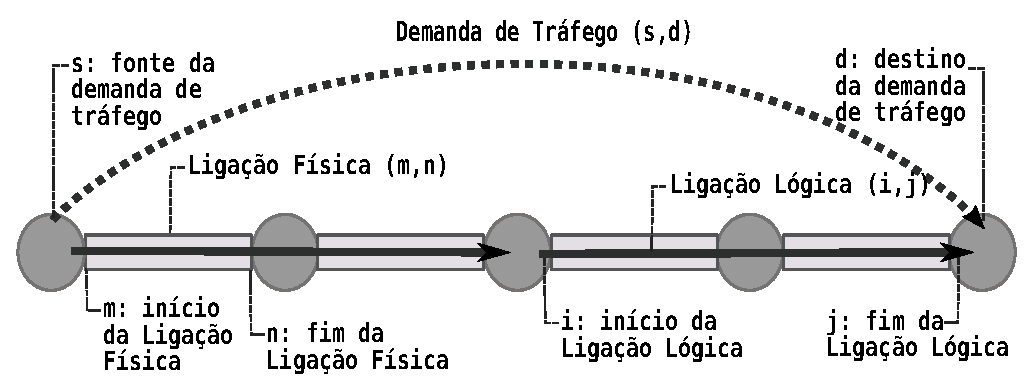
\includegraphics[bb=50 656 565 798, scale=0.8]{figs/indices.eps}
% indices.eps: 1179666x1179666 pixel, 300dpi, 9987.84x9987.84 cm, bb=50 656 565 798
\caption{Representa��o gr�fica da nota��o associada aos n�s da rede.}
\label{fig:Indices}
\end{figure}
% \clearpage

% \subsection{Topologia Generalizada}
% \label{Top}

\zz
\begin{proposition}
\label{Cons}
Uma inst�ncia para o modelo TWA � definida por:

\begin{enumerate}
\item $N$ $=$ N�mero de n�s da rede.
\item $W$ $=$ N�mero m�ximo de comprimentos de onda admitido por fibra.
% \item $H$ $=$ Grau f�sico m�ximo de entrada e sa�da de cada n�.
\item $K$ $=$ Multiplicidade f�sica m�xima admitida entre os pares de n�s.
\item $Cap$ $=$ Capacidade de tr�fego de cada canal l�gico.
% \item $C_{m,n}$ $=$ Custo associado a uma liga��o f�sica orientada entre o par de n�s $(m,n)$.
% \item $T$ $=$ Custo por unidade de fluxo.
\item $P_{s,d}$ $=$ Demanda de tr�fego, com origem $s$ e destino $d$, com $A_s = \sum_d P_{s,d}$.
% \item $A_s = \sum_d P_{s,d}$ $=$ Soma de todas as demandas de tr�fego, com origem $s$.
\end{enumerate}
\end{proposition}

A vari�vel central do modelo, a partir da qual todas as demais ser�o definidas, chamada de \textit{componente da Topologia 
Generalizada} (ou simplesmente \textit{componente topol�gica}), � representada graficamente na Figura \ref{fig:B} e 
formalmente definida na Vari�vel \ref{comp}. Ela sozinha representa as topologias l�gica e f�sica, o trajeto f�sico das 
liga��es l�gicas e o comprimento de onda utilizado. Conforme a terminologia utilizada
neste trabalho daqui por diante, \textit{uma componente topol�gica $B_{i,m,n,w} = k$ � iniciada em $m$, incidente em $n$, com origem $i$,
comprimento de onda $w$ e valor $k$}.


\zz
\begin{theorem}
\label{comp}
 Seja $B_{i,m,n,w} = k\in \{0,..,K\}$, com $i\neq n$, uma componente do conjunto das liga��es l�gicas com origem $i$ e comprimento de onda $w$,
que utilizam $k$ liga��es f�sicas entre os n�s $m$ e $n$.
\end{theorem}

Considerando que $B_{i,m,n,w}=k$ para algum $k \in \{0,..,K\}$, existem $k$ liga��es l�gicas originadas em $i$ no comprimento de onda $w$, passando
por $k$ enlaces f�sicos distintos entre o par de n�s $(m,n)$. Neste caso, cada um desses $k$ enlaces f�sicos ter� que ser uma fibra �ptica distinta
interligando o mesmo par de n�s $(m,n)$, pois haveria interfer�ncia se houvessem dois sinais �pticos originados por fluxos de tr�fego diferentes se
propagando no mesmo sentido, na mesma fibra, com o mesmo comprimento de onda. Note que $K$ limita apenas a multiplicidade dos enlaces f�sicos, ou
seja, o n�mero de fibras �pticas dispostas em paralelo entre dois n�s $(m,n)$. Mesmo que $K=1$, o que torna $B_{i,m,n,w}$ uma vari�vel bin�ria, as
diversas liga��es l�gicas entre um par $(i,j)$ poder�o usar m�ltiplos trajetos f�sicos, ou ainda, mais de um comprimento de onda em uma mesma
fibra. Se ,$\forall i$ , $k=0$ para qualquer $w$, ent�o nenhum enlace f�sico entre o par de n�s $(m,n)$ � utilizado, ou seja $B_{i,m,n,w}=0$, $\forall (i,w)$.

\begin{figure}[hb]
 \centering
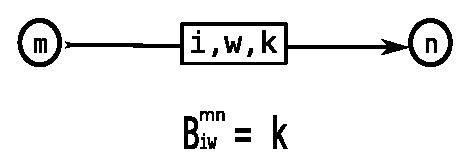
\includegraphics[bb=36 739 246 805, scale=0.7]{figs/B.eps}
% B.eps: 1179666x1179666 pixel, 300dpi, 9987.84x9987.84 cm, bb=36 739 246 805
 \caption{Representa��o gr�fica de uma componente topol�gica.}
 \label{fig:B}
\end{figure}

% \begin{equation}
% s\neq j\quad \text{ e }\quad i\neq j\quad \forall (s,i,j).
% \label{Nules}
% \end{equation}

%A princ�pio, o n�mero de vari�veis do tipo descrito aqui seria $N^3\cdot W$, mas devemos excluir algumas que s�o 
% trivialmente nulas: $s\neq j$ pois $s$ � origem da liga��o l�gica e $j$ � destino da liga��o f�sica; e $i\neq j$ pois n�o s�o 
% aceitos \textit{autoloops} \cite{cormen02}.

% Numa componente da topologia generalizada $B_{i,m,n,w} = k$, o �ndice $i$ representa o n� de origem das $k$ liga��es l�gicas 
% que, passando por uma das liga��es f�sicas iniciadas em $m$ e incidentes em $n$, usa o comprimento de onda $w$.

% \clearpage
\begin{figure}[hb]
 \centering
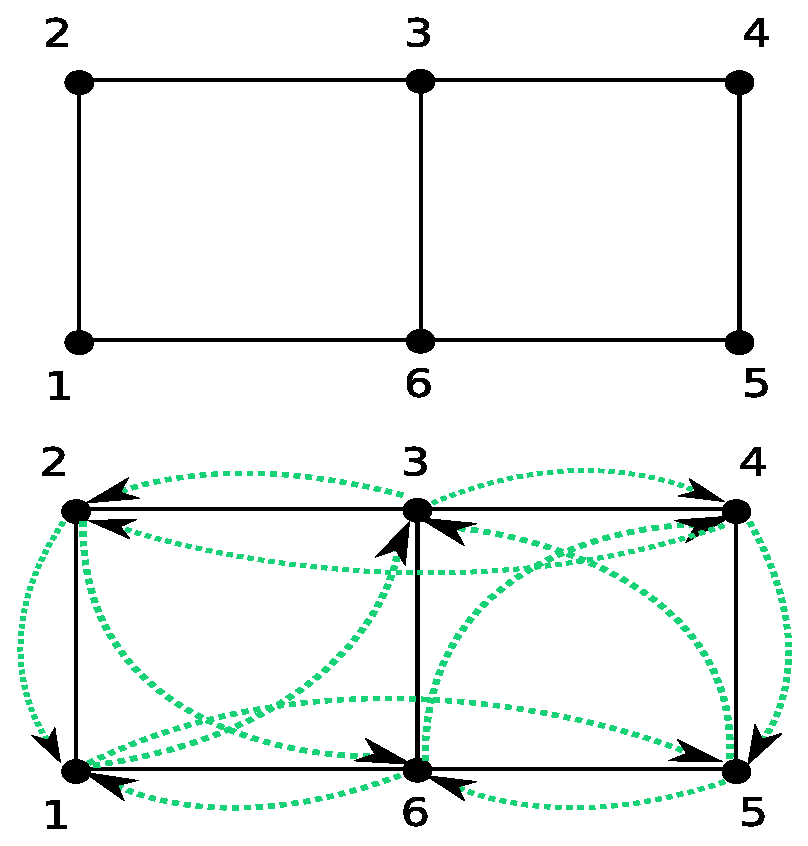
\includegraphics[bb=39 455 511 811, scale=0.6]{figs/topologias.eps}
 % topologias.eps: 1179666x1179666 pixel, 300dpi, 9987.84x9987.84 cm, bb=30 375 511 801
 \caption{Exemplo da interpreta��o das componentes topol�gicas.}
 \label{fig:Tops}
\end{figure}
% \clearpage

 Na Figura \ref{fig:Tops}, temos um exemplo de interpreta��o das componentes topol�gicas, todas com origem no n� $i$ e com o 
mesmo comprimento de onda $w_1$. No item $d)$ desta figura, o valor $2$ da componente que liga os n�s $(i,m)$ � interpretado 
como duas liga��es f�sicas entre esses n�s, representadas no item $a)$. No item $b)$, vemos uma liga��o l�gica dupla entre os 
n�s $(i,n)$, onde uma delas passa de forma transparente pelo n� $m$, como indicado no item $c)$. Note ainda que, no item 
$d)$, h� dois caminhos l�gicos incidentes em $m$ mas apenas um iniciando. Isso indica que uma liga��o l�gica termina em $m$, 
enquanto a outra segue adiante.

% A defini��o das componentes topol�gicas n�o deixa claro aonde terminam as liga��es l�gicas. Sua finaliza��o ser� garantida 
% implicitamente pelas restri��es do modelo. Isso reflete a agrega��o do roteamento dos comprimentos de onda, similar a trabalhos encontradas na
% literatura \cite{Jaumard04}.

A indexa��o atribu�da �s vari�veis $B_{i,m,n,w}$ especificam apenas o n� $i$ onde se iniciam os enlaces l�gicos representados. Isto
significa que estas vari�veis agregam todas as liga��es l�gicas originadas em $i$ que utilizam o enlace f�sico $(m,n)$ e o comprimento de onda $w$,
independente do n� $j$ em que terminam estas liga��es l�gicas. Esta t�cnica consiste em uma abordagem bastante conhecida para a representa��o de
vari�veis em problemas de distribui��o de fluxo em redes. Em \cite{Tornatore07}, este conceito de agrega��o de tr�fego � aplicado como meio de
simplifica��o do modelo, reduzindo substancialmente o n�mero de vari�veis dos problemas resultantes. No TWA, esta agrega��o cumpre o mesmo papel de
simplifica��o, cabendo �s restri��es do modelo garantir implicitamente a termina��o correta destas liga��es l�gicas agregadas nas vari�veis
$B_{i,m,n,w} $.

%  Se $B_{i,m,n,w}=0$, na liga��o f�sica $(m,n)$ (que pode ent�o n�o existir), n�o 
% existem liga��es l�gicas iniciadas em $i$, passando por $(m,n)$, usando o comprimento de onda $w$. Por outro lado, se 
% $B_{i,m,n,w}=k$, para algum $k \in \{0,..,K\}$, existem $k$ liga��es l�gicas originadas em $i$ no 
% comprimento de onda $w$, passando por $k$ liga��es f�sicas distintas entre o par de n�s $(m,n)$ (que agora obrigatoriamente 
% existem). Note que $K$ limita apenas a multiplicidade dos enlaces f�sicos. Mesmo que $K=1$ ( $B_{i,m,n,w}$ ser� uma vari�vel 
% bin�ria), as  liga��es l�gicas entre um par $(i,j)$ poder�o usar m�ltiplos trajetos f�sicos, ou inda, mais de um comprimento 
% de onda em uma mesma fibra.

% A multiplicidade das liga��es l�gicas pode ser controlada por uma restri��o pr�pria, que ser� mostrada na Se��o 
% \ref{ControlMl}.

%  Na vers�o mais enxuta, com a topologia f�sica fixada (veja a Se��o \ref{Fis}, adiante) do modelo � adicionada apenas a 
% vari�vel de distribui��o de fluxo agregado. Dependendo do caso de uso, outras vari�veis podem ser necess�rias (como ser� 
% visto na Se��o \ref{cases}), mas nenhuma supera o n�mero de componentes da topologia generalizada, que define portanto a 
% ordem de grandeza do n�mero de vari�veis desta modelagem.

% \subsection{Conserva��o do Percurso L�gico}
% \label{ConservLogS}

As Vari�veis \ref{FisVar} e \ref{FlowVar} completam as defini��es necess�rias para apresentarmos a forma b�sica do modelo TWA, expresso nas
equa��es de (\ref{ConservLog}) � (\ref{ObjB}).

\zz
\begin{theorem}
\label{FisVar}
 Seja $D_{m,n} \in \{0,..,K\}$ o n�mero de liga��es f�sicas entre o par de n�s $(m,n)$. 
\end{theorem}

\zz
\begin{theorem}
 \label{FlowVar}
 Seja $q_{s,i,j} \in [0,1]$ a fra��o de fluxo originado em $s$, passando pelas liga��es l�gicas entre o par $(i,j)$, com $s\neq j$. 
\end{theorem}

\begin{equation}
 \sum_n B_{i,n,m,w} \geq \sum_n B_{i,m,n,w} ,\quad \forall (i,m,w) \text{, com } i\neq m.
\label{ConservLog}
\end{equation} 

\begin{equation}
\sum_i B_{i,m,n,w} \leq D_{m,n},\quad \forall (m,n,w).
\label{DefFis}
\end{equation} 

% \begin{equation}
% \sum_n D_{m,n} \leq H,\quad \forall m \qquad \text{e} \qquad \sum_m D_{m,n} \leq H,\quad \forall n.
% \label{ConservGFis}
% \end{equation} 

\begin{equation}
\sum_{s} q_{s,i,j}\cdot A_s \leq Cap\cdot (\sum_{m,w} B_{i,m,j,w} - \sum_{n,w} B_{i,j,n,w}),\quad \forall (i,j).
\label{DefCapFlow}
\end{equation} 

\begin{equation}
\sum_j q_{s,s,j} = 1,\, \forall s \quad \text{e} \quad 
\sum_i q_{s,i,d} - \sum_j q_{s,d,j} = \frac{P_{s,d}}{A_s},\, \forall (s,d).
\label{ConservFlow}
\end{equation} 

\begin{equation}
 \label{ObjB}
 \text{Minimize: } \sum_{i,m,n,w} B_{i,m,n,w}.
\end{equation}

A Restri��o (\ref{ConservLog}) garante a continuidade dos percursos e a conserva��o dos comprimentos de onda. Se o n�mero de 
componentes topol�gicas incidentes em $m$ for maior que o n�mero de iniciadas, n�o originadas nele, essa diferen�a � 
o n�mero de liga��es l�gicas que terminam em $m$. � deste modo que a finaliza��o das liga��es l�gicas pode ser mapeada. Isso 
assegura a rastreabilidade das liga��es l�gicas desde sua origem, a partir das componentes topol�gicas agregadas.

%Esta restri��o garante que se h� liga��es l�gicas saindo de um n� $m$, iniciadas em $i$ no comprimento de onda $w$, mas n�o 
% originadas nele ($i\neq m$), ent�o dever� haver (pelo menos) em igual n�mero liga��es l�gicas incidentes em $m$, com a 
% mesma origem e no mesmo comprimento de onda.

% \begin{figure}[htb]
%  \centering
%  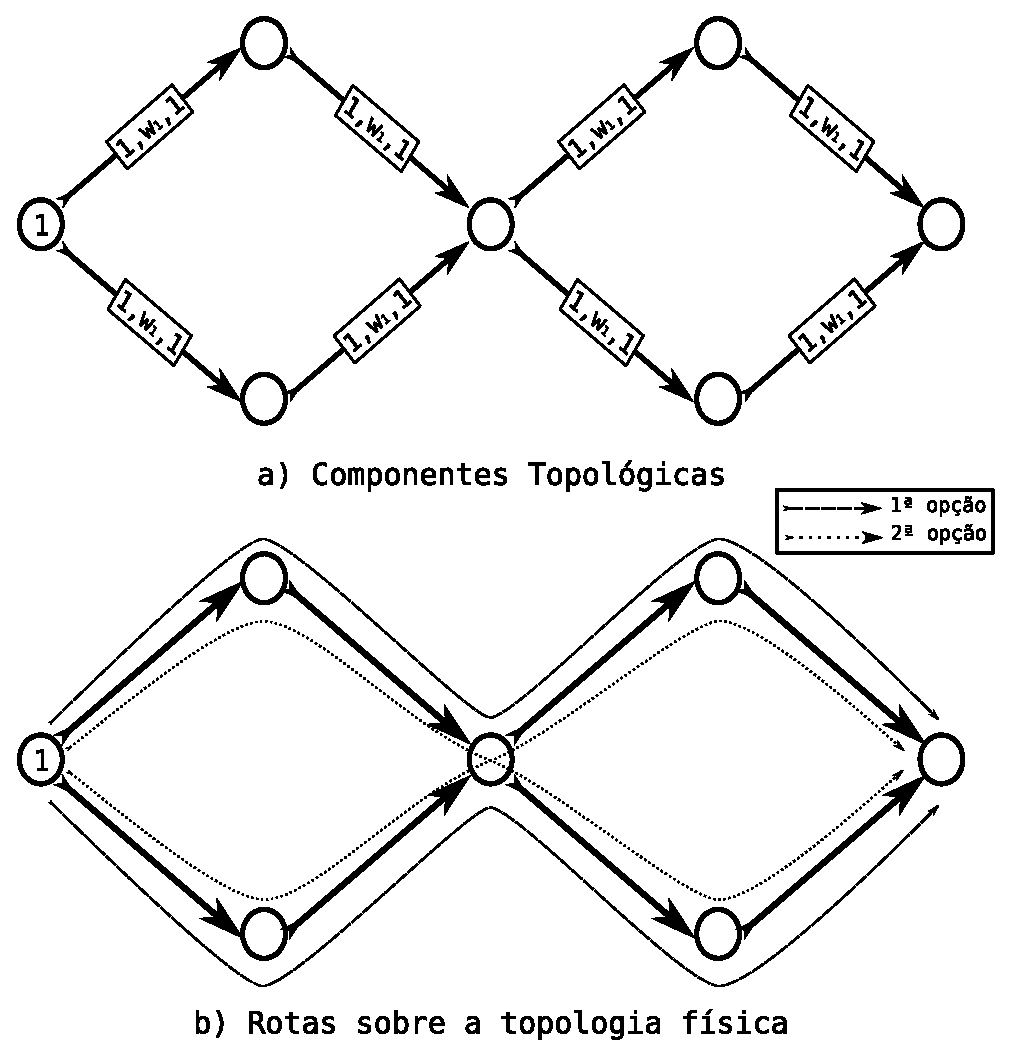
\includegraphics[bb=70 210 533 771, scale=0.5]{figs/unsolved.eps}
%  % unsolved.eps: 1179666x1179666 pixel, 300dpi, 9987.84x9987.84 cm, bb=70 210 533 771
%  \caption{Duas possibilidades de interpreta��o das componentes topol�gicas.}
%  \label{fig:Unsolved}
% \end{figure}
% 
% Isto � suficiente para a modelagem, embora na implementa��o real de m�ltiplas rotas f�sicas entre um mesmo par de n�s 
% $(i,j)$, alguns detalhes ainda carecem ser decididos, pois podem haver mais de uma maneira de configura-los. Um exemplo disso 
% � dado na Figura \ref{fig:Unsolved}, onde o conjunto de componentes topol�gicas dado permite duas possibilidades de 
% configura��o dos percursos l�gicos. Essas situa��es podem ser tratadas considerando outros fatores, como a dist�ncia entre os 
% n�s. Mas s�o quest�es de menor complexidade, se a topologia generalizada j� estiver decidida, e podem ser resolvidas na fase 
% de configura��o da rede. Como isso n�o influencia na modelagem e portanto n�o ser� tratado aqui.
% 
% N�o � evitado explicitamente a ocorr�ncia de ciclos no percurso dos caminhos �pticos, mas isso � indiretamente controlado 
% pela fun��o objetivo, seja ela de minimiza��o de custos, de congestionamento (Se��o \ref{Cong}) ou n�mero de comprimentos de 
% onda utilizados (Se��o \ref{CtrlW}). E mesmo que apare�am ciclos, eles n�o invalidam o resultado.
% 
% \subsection{Topologia F�sica}
% \label{Fis}

Apesar da topologia f�sica ser determinada pelas componentes da topologia generalizada, para fins de controle do custo de instala��o da rede f�sica, 
s�o necess�rias novas inc�gnitas. Para este fim, � definida a Vari�vel \ref{FisVar}, que registra em $D_{m,n}$ a multiplicidade f�sica alcan�ada pelas
componentes topol�gicas. Se $D_{m,n}=0$, n�o h� liga��es f�sicas entre o 
par $(m,n)$, mas se $D_{m,n}=k$, para algum $k \in \{0,..,K\}$, existem $k$ liga��es f�sicas entre o par $(m,n)$. Pela forma como $D_{m,n}$ �
calculada na Restri��o \ref{FisVar}, a rigor, seu valor poderia ser maior do que � determinado pelas componentes topol�gicas. Mas isso n�o ocorre pois o n�mero
de liga��es f�sicas ser� minimizado na fun��o objetivo.

Se $D_{m,n}$ for dado de entrada do problema, a Restri��o (\ref{DefFis}) limita a multiplicidade f�sica das componentes topol�gicas 
$B_{i,m,n,w}$. Ainda neste caso, se $D_{m,n}=0$ para um certo par $(m,n)$, devem ser retiradas da modelagem as vari�veis $B_{i,m,n,w}$ correspondentes. Isto deve
ser considerado em todo o modelo e daqui por diante toma-se como subentendido.

% Se a topologia f�sica � livre, a Restri��o (\ref{ConservGFis}) � necess�ria para o controle do grau f�sico de 
% sa�da e entrada em cada n�, caso contr�rio esta restri��o pode ser desconsiderada.

%Quando a topologia f�sica � livre, n�o � controlada a exist�ncia de $D_{i,j}\neq 0$, com $B_{s,i,j,w}=0$, $\forall (s,w)$. 
% Dependendo do caso de uso, isso ou n�o influencia no resultado, ou pode ser controlado indiretamente pela fun��o objetivo, 
% por exemplo, por meio do custo de instala��o. Opcionalmente poderia-se usar para este fim uma restri��o da forma $\sum_{s,w} 
% B_{s,i,j,w} \geq D_{i,j}$, para todo $(i,j)$, mas essa hip�tese � por hora desconsiderada.

% \subsection{Controle de Fluxo}
% \label{Flow}

Para resolver o sub-problema de roteamento de tr�fego, s�o definidas as vari�veis de fra��o de fluxo agregado (Vari�vel \ref{FlowVar}), utilizadas
na Restri��o (\ref{DefCapFlow}). Como podem haver m�ltiplas liga��es l�gicas entre um par $(i,j)$, o tr�fego 
entre um par de n�s dever� ser limitado pela capacidade de uma liga��o l�gica multiplicada pelo n�mero de liga��es l�gicas em quest�o. Na
Restri��o \ref{DefCapFlow}, este n�mero � representado, para as liga��es l�gicas entre o par $(i,j)$, como a
quantidade de componentes topol�gicas incidentes em $j$ ({\footnotesize$\sum_{m,w}B_{i,m,j,w}$}), diminu�do do n�mero de componentes
topol�gicas iniciadas em $j$ ({\footnotesize$\sum_{n,w}B_{i,j,n,w}$}).

% Esse n�mero, na Restri��o \ref{DefCapFlow}, � obtido da quantidade de componentes topol�gicas originadas em $i$ e incidentes em $j$, diminu�do do
% n�mero de componentes topol�gicas iniciadas em $j$ e originadas em $i$. 

A conserva��o de fluxo � assegurada pela Restri��o (\ref{ConservFlow}), que tamb�m garante o envio e a entrega das demandas 
de tr�fego. As equa��es da Restri��o (\ref{ConservFlow}) s�o semelhantes, em sua forma, �s encontradas na modelagem agregada 
para o VTD \cite{ram02}. Todavia, sua interpreta��o � sutilmente diferente, pois aqui uma determinada fra��o de fluxo de tr�fego pode ser subdividida e
transportada simultaneamente por mais de uma liga��o l�gica entre o par $(i,j)$. Por exemplo, em comprimentos de onda diferentes em um mesmo enlace
f�sico $(m,n)$ que interliga diretamente $(i,j)$, ou por rotas f�sicas disjuntas entre os n�s $(i,j)$, neste �ltimo caso, independente do
comprimento de onda.

% \subsection{Saltos F�sicos}

Uma m�trica importante para o projeto de redes �pticas � o n�mero de saltos f�sicos da topologia \cite{Zang00}. Este valor 
� minimizado na Fun��o Objetivo (\ref{ObjB}), atrav�s da soma de todas as componentes topol�gicas, pois cada componente 
topol�gica representa um salto f�sico. Uma propriedade importante desta abordagem � que ela evita o aparecimento de 
ciclos na topologia generalizada. O ideal seria minimizar a dist�ncia percorrida por cada enlace l�gico, o que controlaria a degrada��o do sinal �ptico.
Minimizar o n�mero total de saltos foi adotado por uma quest�o de compatibilidade com os resultados encontrados em \cite{Karcius04}, que ser�o usados na
compara��o dos experimentos computacionais da Se��o \ref{testes}.

Como o n�mero de componentes topol�gicas � $N�\cdotp W$ e o n�mero de restri��es � $\Theta(N�\cdotp W)$, o n�mero de vari�veis do modelo � da ordem de
$\Theta(N�\cdotp W)$. Quando a topologia f�sica � um dado de entrada, sendo $H$ o n�mero total de liga��es f�sicas da rede, ent�o o n�mero de 
componentes da topologia generalizada ser� $N\cdotp H\cdotp W$, portanto, o n�mero de vari�veis do modelo ser� $\Theta(N\cdotp H\cdotp W)$, semelhante aos modelos
mais enxutos para resolver apenas o RWA \cite{Jaumard04}.


\subsection{Liga��es L�gicas em cada Fibra e Grau L�gico}

Dada a abrang�ncia do modelo b�sico, diversas m�tricas poderiam ser controladas ou diretamente minimizadas, conforme a aplica��o.
Apresentamos agora como podem ser inclu�dos dois par�metros de 
controle bem conhecidos e que ser�o utilizados nos experimentos computacionais da Se��o \ref{testes}.

No modelo TWA o n�mero de liga��es l�gicas � implicitamente limitado pela capacidade f�sica do n� $m$ de realizar liga��es l�gicas, que � a
capacidade do \textit{Optical switch} de receber ou originar conex�es \cite{Zang00}. Todavia, o n�mero de transceptores em um n�, pode ser menor
que essa capacidade \cite{Zang00,ram02}. Assumimos que todos os n�s tem o mesmo n�mero 
de transceptores, que � chamado de grau l�gico ($Gl$), que tamb�m passa a ser um dado de entrada. Para controlar 
o grau l�gico de sa�da e entrada em cada n�, � necess�ria a Restri��o \ref{ConservGl}, que deve ser adicionada ao modelo b�sico. 

Outro controle muito usado nas modelagens de RWA , � o n�mero m�ximo de 
liga��es l�gicas por fibra  $L$ (Dados \ref{adicionais}) \cite{Zang00,Jaumard04}. Este par�metro limita a densidade da multiplexa��o de
comprimentos de onda por enlace f�sico, um importante aspecto de Redes �pticas WDM. Este limite � implementado pela Restri��o (\ref{L}).

\zz
\begin{proposition}
Constantes adicionais:
\begin{enumerate}
 \item $Gl$ $=$ Grau L�gico.
 \item $L$ $=$ N�mero m�ximo de liga��es l�gicas em cada fibra.
\end{enumerate}
\label{adicionais}
\end{proposition}

\begin{equation}
\sum_{w,n} B_{m,m,n,w} \leq Gl,\quad \text{e}\quad 
\sum_{i,n,w} B_{i,n,m,w} - \sum_{i,n,w} B_{i,m,n,w} \leq Gl,\quad \forall m \text{, com } i\neq m.
\label{ConservGl}
\end{equation} 

\begin{equation}
 \label{L}
\sum_{i,w} B_{i,m,n,w}\leq L,\quad \forall (m,n).
\end{equation}





%%%%%%%%%%%%%%%%%%%%%%%%%%%%%%%%%%%%%
%% Adapta��es do Modelo B�sico
%% Copyright 2009 Fabio de Oliveira Lima.
%% Este documento � distribu�do nos termos da licen�a 
%% GNU General Public License v2.
%%%%%%%%%%%%%%%%%%%%%%%%%%%%%%%%%%%%%


\chapter{Adapta��es do Modelo B�sico}
\label{cases}

Neste cap�tulo s�o apresentados outros casos de uso da modelagem TWA. Dada a abrang�ncia do modelo b�sico, diversas m�tricas poderiam ser controladas ou
diretamente minimizadas, conforme a aplica��o. Apresentamos agora como podem ser inclu�dos par�metros de controle bem conhecidos, alguns deles ser�o utilizados
nos experimentos computacionais das Se��es \ref{cap:testes-sec:karcius} e \ref{cap:testes-sec:sivarajan}.


Veremos, por exemplo, como incluir as restri��es de controle do grau l�gico dos n�s e como usar o congestionamento como fun��o objetivo, duas considera��es
comuns das modelagens de VTD \cite{ram02}. O grau l�gico de entrada ou de sa�da de um n� � o n�mero m�ximo de liga��es l�gicas que podem se originar ou
terminar nele, respectivamente. Fixado um valor de grau l�gico para a rede, todos os n�s dever�o ter o mesmo valor de grau l�gico de entrada e sa�da. O
congestionamento � a quantidade de tr�fego designado ao caminho �ptico mais carregado da rede. Ao minimizar o congestionamento a tend�ncia � distribuir
igualmente o tr�fego entre todos os caminhos �pticos. Este crit�rio garante que n�o haja subutiliza��o ou sobrecarga nos enlaces l�gicos que formam a
topologia virtual da rede. A sobrecarga causa aumento do atraso em filas e consequente diminui��o do vaz�o \cite{ram02}.

Ser�o mostradas tamb�m formas de controlar ou otimizar o n�mero de comprimentos de onda, entre outras m�tricas normalmente vistas em modelos de RWA
\cite{Zang00}.

% Algumas vezes ao longo desta se��o ser� necess�rio considerar a capacidade f�sica do n� $m$ de realizar liga��es l�gicas 
% (Dados \ref{CapLogi}), que � a capacidade do \textit{Optical switch} de receber ou originar liga��es \cite{Zang00}. 
% 
% \zz
% \begin{dados}
% Se a topologia f�sica � uma vari�vel do modelo ($D_{mn}$), o grau f�sico de entrada e sa�da $H$ � considerado uniforme para 
% a rede e $CapLog_m = H\cdot W$. Caso seja de interesse fixar a topologia f�sica, passando a mesma como par�metro do modelo, 
% $CapLog_m = \sum_n D_{m,n}\cdot W$.\label{CapLogi}
% \end{dados}

\section{Grau L�gico e Multiplicidade de Liga��es L�gicas}
\label{ConservGl}

No modelo b�sico do TWA o n�mero de liga��es l�gicas n�o � limitado, mas � controlado indiretamente pelos custos de instala��o e pelo n�mero de comprimentos de
onda por fibra, ou ainda, caso a topologia f�sica seja um dado de entrada, pelo n�mero de liga��es f�sicas existentes. 

Caso se queira fazer esse controle diretamente, ser�o considerados os dados de entrada $GLin_m$ e $GLout_m$, respectivamente, os graus l�gicos de entrada e
sa�da do n� $m$.  

Para controlar o grau l�gico, s�o necess�rias duas restri��es que devem ser adicionadas ao modelo b�sico: a Restri��o (\ref{ConservGLout}) 
que controla o grau l�gico de sa�da; e a Restri��o (\ref{ConservGLin}) que controla o grau l�gico de entrada.

A Restri��o (\ref{ConservMl}) acrescenta a limita��o da multiplicidade das liga��es l�gicas ($Ml$) ao modelo TWA, que � 
indiretamente limitada pelo grau l�gico. Para n�o usar multiplicidade nas liga��es l�gicas, basta fazer 
$Ml=1$. 

% \zz
\begin{dados} Constantes adicionais: 
 \begin{enumerate}
\item Grau L�gico de entrada do n� $m$ $=$ $GLin_m, \quad \forall m$.
\item Grau L�gico de sa�da do n� $m$ $=$ $GLout_m, \quad \forall m$.
\item $Ml$ $=$ Multiplicidade das Liga��es L�gicas.                                              
\end{enumerate}
\label{Gl-Ml}
\end{dados}

\begin{equation}
\sum_{wn} B_{mw}^{mn} \leq GLin_m\Forall{m},\, \mbox{\small$i\neq m$} 
\label{ConservGLin}
\end{equation} 

\begin{equation}
\sum_{inw} B_{iw}^{nm} - \sum_{inw} B_{iw}^{mn} \leqslant GLout_m\Forall{m},\, \mbox{\small$i\neq m$} 
\label{ConservGLout}
\end{equation} 

\begin{equation}
\sum_{nw} B_{iw}^{nm} - \sum_{nw} B_{iw}^{mn} \leqslant Ml\Forall{(i,m)},\, \mbox{\small$i\neq m$}
\label{ConservMl}
\end{equation}


% \section{Custos de Instala��o e Opera��o}
% \label{ObjC}
% 
% Uma m�trica importante no projeto da redes �pticas � a minimiza��o dos custos de instala��o e opera��o \cite{mukherjee}. O 
% custo de instala��o $C_{m,n}$ � o custo associado a uma liga��o f�sica orientada entre o par de n�s $(m,n)$. O custo de 
% opera��o $T$ � definido como o custo por unidade de fluxo. Este �ltimo pode ser dividido em duas partes, uma constante ($Tc = 
% \sum_{s,d} T\cdot P_{s,d}$), formada pelas demandas de tr�fego (que necessariamente dever�o ser roteadas), e outra vari�vel 
% ($Tv = \sum_{s,i,j} T\cdot q_{s,i,j}\cdot A_s $), composta pelo tr�fego adicional que � gerado, ou seja, o tr�fego 
% retransmitido.
% 
% Por essa raz�o, minimizar o custo por unidade de fluxo � equivalente a minimizar o tr�fego retransmitido na rede, o que por 
% sua vez, equivale a minimizar o processamento eletr�nico de tr�fego dos n�s da rede \cite{Renato06}. Soma-se a isso o fato de 
% que � necess�ria nesta modelagem a Restri��o (\ref{DefCapFlow}), de limita��o da capacidade $Cap$ dos canais l�gicos. Deste 
% modo, limitando o congestionamento na rede e minimizando o processamento, temos uma abordagem mais eficiente, quanto ao custo 
% computacional, para o projeto da topologia virtual em compara��o com a minimiza��o do congestionamento da rede 
% \cite{Renato06, ram02}. 
% 
% Se n�o for necess�rio ponderar o custo por unidade de fluxo, basta fazer $T=1$, e se n�o for necess�rio considerar o custo 
% total de instala��o ($CI = \sum_{m,n} C_{m,n}\cdot D_{m,n}$), basta fazer $C_{m,n}=0$ para todo $(m,n)$. Deste modo seria 
% simplesmente um modelo de minimiza��o do processamento, com limita��o do congestionamento \cite{Renato06}. A fun��o objetivo, 
% que � a minimiza��o do custo total $R = CI + Tc + Tv$, � dada explicitamente pela restri��o a seguir.
% 
% \begin{equation}
%  \text{Minimize: } R =  CI + Tc + Tv = \sum_{m,n} C_{m,n}\cdot D_{m,n} + \sum_{s,d} T\cdot P_{s,d} + 
% \sum_{s,i,j} T\cdot q_{s,i,j}\cdot A_s.
% \label{MinC}
% \end{equation} 


\section{Congestionamento}
\label{Cong}

Como foi comentado na Se��o \ref{Basic}, a multiplicidade das liga��es l�gicas fica impl�cita para as vari�veis de 
distribui��o de tr�fego. Deste modo, n�o � poss�vel minimizar diretamente o tr�fego em cada canal. Portanto, para minimizar o 
congestionamento mantendo esta multiplicidade, s�o necess�rias novas vari�veis para contabilizar o tr�fego em cada canal.

A fra��o de tr�fego $f_{i,r,j}$ (Vari�vel \ref{f}) � semelhante a Vari�vel \ref{FlowVar} (fra��o de fluxo), com a diferen�a 
de que a Vari�vel \ref{f} separa o fluxo por canal, e a anterior considerava todos os canais. Por sua vez, a liga��o l�gica 
$F_{i,r,j}$ (Vari�vel \ref{F}) mapeia cada canal �ptico em uma liga��o l�gica independente. 

Mas para isso, precisamos que sejam definidos os graus l�gicos para os n�s da rede. E tamb�m ser�o necess�rias as Restri��es (\ref{ConservGLin}) e
(\ref{ConservGLout}), para controle de grau l�gico.

% \zz
\begin{notation}
O �ndice $r\in\{1,\cdots,CapLog_{mn}\}$ enumera os poss�veis m�ltiplos canais l�gicos entre par $(m,n)$, onde $CapLog_{m,n}$ 
� o m�nimo entre $GLout_m$ e $GLin_n$. 
\label{indice:r}
\end{notation}

% \zz
\begin{var}
Fra��o de Tr�fego $=$ $f_{irj} \in [0,1]$: vari�vel cont�nua.
 \label{f}
\end{var}

% \zz
\begin{var}
Liga��o L�gica $=$ $F_{irj} \in \{0,1\}$: vari�vel bin�ria.
 \label{F}
\end{var}

% \zz
\begin{var}
 \label{FmaxVar}
$F_{max}$ $=$ Fra��o de tr�fego do canal mais carregado da rede (congestionamento).
\end{var}


\begin{equation}
 \sum_{nw} B_{iw}^{nm} - \sum_{nw} B_{iw}^{mn} = \sum_r F_{irm}\Forall{(i,m)} \text{, com } i\neq m.
\label{DefChLog}
\end{equation}

\begin{equation}
F_{irj} \geqslant f_{irj} \Forall{(i,r,j)}.
\label{DefChFlow}
\end{equation}

\begin{equation}
\sum_{sw} q_{sw}^{ij}\cdot A_s = Cap\cdot (\sum_r f_{irj})\Forall{(i,j)}.
\label{DefCapFlowCh}
\end{equation}

\begin{equation}
F_{max} \geqslant f_{irj}\Forall{(i,r,j)}.
\label{DefFmax}
\end{equation}

\begin{equation}
\text{Minimize: } F_{max}.
\label{ObjFmax}
\end{equation}

A Restri��o (\ref{DefChLog}) determina as liga��es l�gicas $F_{irj}$ em termos dos componentes topol�gicos. Em seguida, a 
Restri��o (\ref{DefChFlow}) define a fra��o do tr�fego em cada canal, limitado pela exist�ncia do canal. Para as vari�veis 
definidas nesta se��o, � necess�ria uma restri��o de limita��o da capacidade (\ref{DefCapFlowCh}) adicional. 
Por fim, definimos o congestionamento ($F_{max}$) na Vari�vel \ref{FmaxVar} e a Restri��o 
(\ref{DefFmax}) determina $F_{max}$ em termos das fra��es de tr�fego em cada canal. Deste modo, a Fun��o Objetivo 
(\ref{ObjFmax}) agora consiste em minimizar $F_{max}$. Apesar das novas vari�veis introduzidas nesta se��o, a ordem de 
grandeza no n�mero de vari�veis continua sendo comandada pelos componentes topol�gicos. 

O caso de uso apresentado nesta se��o, mostra que � poss�vel minimizar diretamente o congestionamento nesta modelagem, pois 
esta � uma bem conhecida m�trica para o VTD. Todavia, uma abordagem mais eficiente � a simples limita��o do congestionamento, 
minimizando outra m�trica, de modo a deixar o modelo mais trat�vel \cite{Renato06}, como foi usado na forma b�sica do modelo 
TWA.

Uma forma alternativa, e bem mais simples, para se minimizar diretamente o congestionamento � adotando a Restri��o
(\ref{ConservMl}), com $Ml=1$. Todavia, perdendo assim a capacidade de se obter solu��es com liga��es l�gicas m�ltiplas. 
Deste modo, pode-se minimizar o congestionamento adotando apenas a Restri��o (\ref{Hmax}), al�m da Vari�vel (\ref{FmaxVar}) e a Fun��o Objetivo (\ref{ObjFmax}).

\begin{equation}
F_{max} \geqslant \sum_{sw} q_{sw}^{ij}\cdot A_s\Forall{(i,j)} \text{, } Ml=1
\label{Hmax} 
\end{equation}




\section{Liga��es L�gicas em cada Fibra}
\label{LimW}

Um controle muito usado nas modelagens de RWA  \cite{Zang00,Jaumard04}, � o n�mero m�ximo L de 
liga��es l�gicas por fibra, Vari�vel (\ref{LimWd}). Ela limita a densidade da multiplexa��o de
comprimentos de onda por enlace f�sico, um importante aspecto de Redes �pticas WDM. Caso seja fixada, ela pode ser usada para limitar cada liga��o f�sica, como �
feito pela Restri��o (\ref{L}), ou minimizado diretamente como fun��o objetivo. Caso a Restri��o (\ref{L}) seja adotada, ela tamb�m limitar� a capacidade 
f�sica dos n�s realizarem liga��es l�gicas.


% \zz
\begin{var}
 \label{LimWd}
$L$ $=$ N�mero m�ximo de liga��es l�gicas em cada fibra.
\end{var}

\begin{equation}
 \label{L}
\sum_{iw} B_{iw}^{mn}\leqslant L\Forall{(m,n)}.
\end{equation}


\section{N�mero de Saltos F�sicos}

Uma m�trica importante para o projeto de redes �pticas � o n�mero de saltos f�sicos da topologia \cite{Zang00}. Este valor 
� minimizado na Fun��o Objetivo (\ref{Obj:B}), atrav�s da soma de todos os componentes topol�gicos, pois cada componente 
topol�gico representa um salto f�sico. Uma propriedade importante desta abordagem � que ela evita o aparecimento de 
ciclos na topologia. O ideal seria minimizar a dist�ncia percorrida por cada enlace l�gico, o que controlaria a degrada��o do sinal �ptico.
Minimizar o n�mero total de saltos pode ser adotado por uma quest�o de compatibilidade com outros modelos, como os resultados encontrados em \cite{Karcius04}, que
ser�o usados na compara��o dos experimentos computacionais do Cap�tulo \ref{cap:testes-sec:karcius}.

\begin{equation}
 \label{Obj:B}
 \text{\small Minimize: } \sum_{imnw} B_{iw}^{mn}.
\end{equation}

As vari�veis de fra��o de fluxo agregado, definidas no modelo b�sico, s�o suficientes para modelar a distribui��o do tr�fego, embora na implementa��o real de
m�ltiplas rotas f�sicas entre um mesmo par de n�s $(i,j)$, alguns detalhes ainda carecem ser decididos, pois podem haver mais de uma maneira de configura-los. Um
exemplo disso � dado na Figura \ref{fig:Unsolved}, onde o conjunto de componentes topol�gicos dado permite duas possibilidades de 
configura��o dos percursos l�gicos. � garantida implicitamente a aloca��o de recursos suficientes, mas este sub-problema fica sem ser resolvido pelo modelo. 
Por essa raz�o, n�o � poss�vel controlar a real dist�ncia percorrida pelas demandas de tr�fego, sendo este um preju�zo da
modelagem TWA.

Essas situa��es podem ser tratadas considerando outros fatores, como a dist�ncia entre os 
n�s. Mas s�o quest�es de menor complexidade, se a topologia j� estiver decidida, e podem ser resolvidas na fase 
de configura��o da rede. Isso n�o influencia na modelagem dos recursos da rede e portanto n�o ser� tratado aqui.

\begin{figure}[htb]
 \centering
 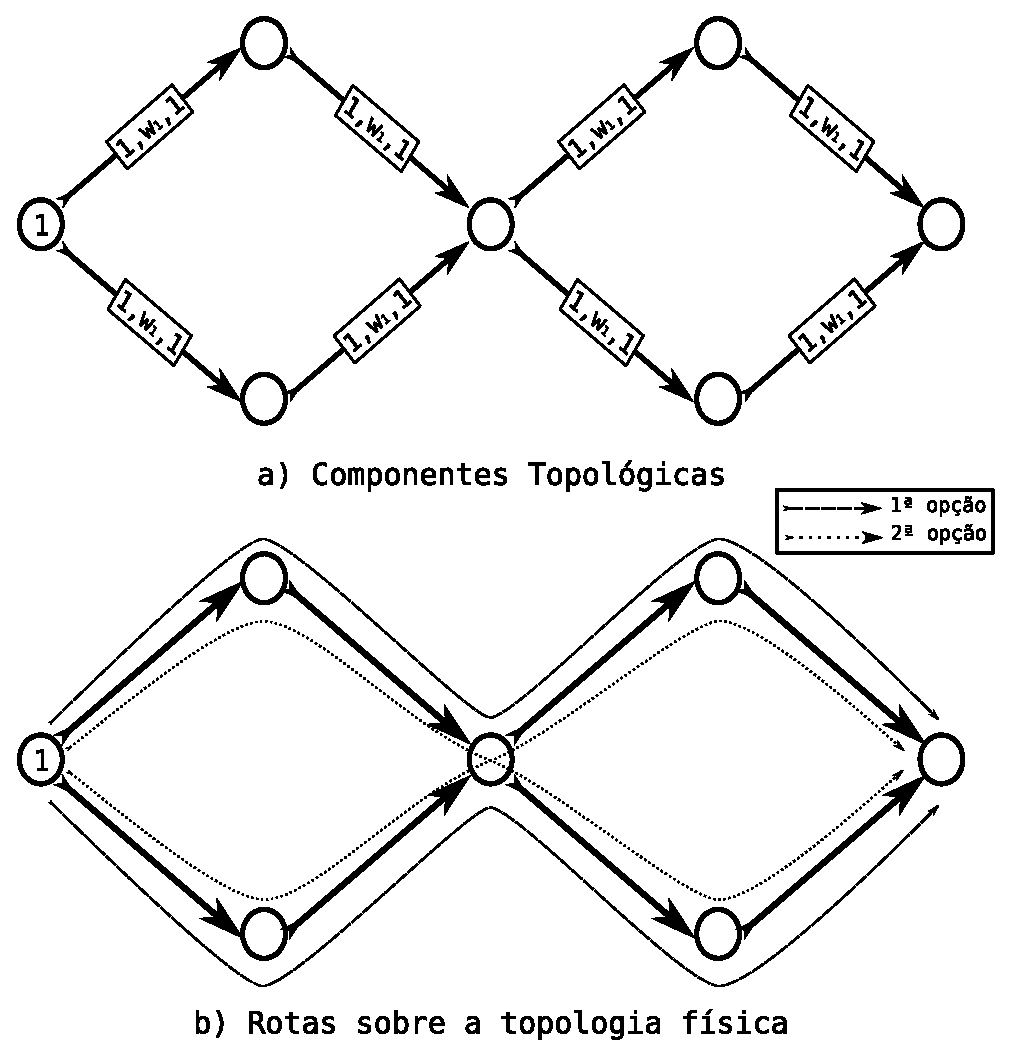
\includegraphics[bb=71 267 541 759, scale=0.8]{figs/unsolved.eps}
 % unsolved.eps: 1179666x1179666 pixel, 300dpi, 9987.84x9987.84 cm, bb=70 210 533 771
 \caption{Em $b)$ vemos duas poss�veis de interpreta��es dos componentes topol�gicos em $a)$.}
 \label{fig:Unsolved}
\end{figure}


\section{Comprimentos de Onda}
\label{CtrlW}

Um objetivo comum nas modelagens do RWA � controlar o n�mero de comprimentos de onda utilizados na rede \cite{Zang00, 
Jaumard04}. Para determinar se um comprimento de onda foi usada na rede, temos a Restri��o (\ref{DefQw}), que limita a soma 
de todos os componentes topol�gicos no comprimento de onda $w$, pela exist�ncia de $Q_w$ (Vari�vel \ref{Cw}). O fator $M\cdot 
(N� - N)$ representa o n�mero m�ximo de componentes topol�gicos que podem usar o comprimento de onda $w$ ao mesmo tempo. Ela 
deve ser adicionada �quelas do modelo TWA, mas somente no caso da topologia f�sica ser livre. 

Pois o n�mero de caminhos que um comprimento de onda pode ter entre um mesmo par $(i,j)$ � a multiplicidade f�sica da 
rede, onde $(N� - N)$ � o n�mero de pares $(i,j)$ poss�veis, e $M$ � a multiplicidade f�sica da rede. Qualquer n�mero maior 
do que este tamb�m manteria a integridade da restri��o, todavia, restri��es mais precisas podem ajudar os algoritmos de 
resolu��o de modelos MILP. 

Caso a topologia f�sica seja fixada, h� a Restri��o (\ref{DefFisQw}) que � mais conveniente, pois deixaria o modelo mais enxuto. Caso a 
topologia f�sica da rede seja um dos dados de entrada, h� uma forma alternativa para se definir $Q_w$, que reaproveita uma 
das restri��es do modelo TWA. Deixando assim de acrescentar uma nova restri��o ao modelo. Com $D_{mn}$ fixo, podemos 
multiplic�-lo por $Q_w$ na Restri��o (\ref{DefFis}), sem prejudicar a fun��o original da equa��o, e obter o mesmo efeito da 
Restri��o (\ref{DefQw}). Deste modo, a Restri��o (\ref{DefFisQw}) deve substituir a equa��o (\ref{DefFis}) do modelo 
original. Para minimizar diretamente o n�mero de comprimentos de onda utilizados na rede, basta usar a soma de todas as 
vari�veis $Q_w$ (Vari�vel \ref{Cw}) como fun��o objetivo.

% Opcionalmente pode-se limitar o processamento, controlando o valor de $Tv$, como foi definido na Se��o \ref{ObjC}. Para isso � necess�rio incluir um
% \textit{bound} para o processamento e a restri��o adicional (\ref{TcUb}). A limita��o do congestionamento ainda pode continuar sendo feita pela Restri��o
% (\ref{DefCapFlow}).

% \zz
% \begin{proposition}
%  \label{TcUperBound}
% $TcUb$ $=$ \textit{Uper Bound} para o processamento.
% \end{proposition}

% \zz
\begin{var}
 \label{Cw}
Seja $Q_w\in\{0,1\}$, com $w \in \{1,..,W\}$. $Q_w = 1$ se 0 comprimento de onda $w$ � utilizada na rede e $Q_w = 0$, caso contr�rio.
\end{var}

\begin{equation}
 \label{DefQw} 
\sum_{imn} B_{iw}^{mn} \leqslant M\cdot (N� - N)\cdot Q_w\Forall{w}.
\end{equation}

\begin{equation}
\sum_i B_{iw}^{mn} \leqslant Q_w\cdot D_{mn}\Forall{(m,n,w)}.
\label{DefFisQw}
\end{equation} 

% \begin{equation}
%  \label{TcUb}
% TcUb \geq \sum_{s,d,m} T\cdot q_{s,d,m}\cdot A_m.
% \end{equation}

\begin{equation}
 \label{ObjW}
\text{Minimize: } \sum_w Q_w.
\end{equation}


\section{Convers�o de Comprimentos de Onda}
\label{Conv}

Outro cen�rio comum nas modelagem para o RWA � a possibilidade de convers�o do comprimento de onda ao longo de um caminho �ptico. H� 
duas formas mais comuns de se tratar essa abordagem. Ou um n� possui capacidade total de convers�o \cite{Zang00, Jaumard04, Tornatore07} e todas 
as liga��es l�gicas passando por ele podem mudar de comprimento de onda nessa passagem, ou h� uma quantidade m�xima de convers�es \cite{ram98, 
Karcius04}. Como o primeiro m�todo � apenas um caso particular do segundo, trataremos do caso mais geral.

N�o ser� fixado quais n�s ter�o a capacidade de convers�o, mas sim controlaremos o n�mero de convers�es na rede, pela Vari�vel \ref{x}. Caso a topologia f�sica
seja vari�vel, � necess�rio definir um limite para o n�mero de liga��es f�sicas originadas em cada n� da rede.

\begin{dados}
 $GFout_m$ $=$ N�mero m�ximo de liga��es f�sicas originadas no n� $m$.
\end{dados}

\begin{var}
 \label{x}
O n�mero de convers�es em um n� $m$, de um comprimento de onda $w$, realizadas nas liga��es l�gicas originadas em $i$, � mapeado pela vari�vel 
$x_{imw}$. Onde $x_{imw} \in \{0, \cdots, GFout_m\}$, se a topologia f�sica � livre, ou $x_{imw} \in \{0, \cdots, \sum_n D_{mn}\}$, caso 
$D_{mn}$ seja um par�metro. 
\end{var}

Se a topologia f�sica � fixa, ent�o $x_{imw}$ j� est� bem definida, caso contr�rio, ser� necess�ria a restri��o adicional (\ref{Defx}).

\begin{equation}
 \label{Defx}
x_{imw} \leq \sum_n D_{mn}\Forall{(i,m,w)}.
\end{equation}

Ao se habilitar um n� a realizar convers�es de comprimento de onda, torna-se necess�rio utilizar uma restri��o mais geral, que garante a conserva��o fixada a
origem, mas independente do comprimento de onda. A Restri��o (\ref{ConservLogC}) cumpre esse papel. Ela sozinha j� habilita o n� com capacidade de convers�o
total, onde todo comprimento de onde que chega pode ser convertido livremente. J� o n�mero de convers�es � mapeado pela Restri��o (\ref{ConservLogCx}), que
substitui a Restri��o (\ref{DefCapFlow}).

\begin{equation}
 \label{ConservLogC}
 \sum_{nw} B_{iw}^{nm} \geq \sum_{nw} B_{iw}^{mn}\Forall{(i,m)} \text{, com } i\neq m.
\end{equation}


\begin{equation}
 \label{ConservLogCx}
 \sum_{s} q_{sw}^{ij}\cdot A_s \leqslant Cap\cdot \left(\sum_{m} B_{iw}^{mj} - \sum_{n} B_{iw}^{jn} - x_{ijw}\right) \Forall{(i,j,w)}
\end{equation}

Note na defini��o da Vari�vel \ref{x}, que o comprimento de onda de sa�da do conversor n�o � registrada. A Restri��o (\ref{ConservLogCx}) 
assegura que haver� componentes topol�gicos no comprimento de onda $w$, com origem $i$, chegando em $m$ em n�mero suficiente para realizar as 
convers�es. Para cada uma destas, a Restri��o (\ref{ConservLogC}) garante que haver� algum componente partindo de $m$, com origem $i$, mas em um 
comprimento de onda diferente de $w$. Aqui tamb�m podem ocorrer situa��es como a que foi ilustrada na Figura \ref{fig:Unsolved}, nas quais algo 
fica indefinido na interpreta��o dos componentes. Mas esses casos tamb�m n�o influenciam na modelagem e por isso tamb�m n�o ser�o aqui 
considerados.

Pode ser conveniente limitar o n�mero de convers�es em cada n�, ou seja, limitar a soma $\sum_{iw} x_{imw}$, ou o n�mero total de convers�es. 
Ou ainda, usar este �ltimo como fun��o objetivo, o que � feito pela Restri��o (\ref{ObjX}).

\begin{equation}
 \label{ObjX}
 \text{Minimize: } \sum_{imw} x_{imw}.
\end{equation}




%%%%%%%%%%%%%%%%%%%%%%%%%%%%%%%%%%%%%
%% Lower Bounds
%% Copyright 2009 Fabio de Oliveira Lima.
%% Este documento � distribu�do nos termos da licen�a 
%% GNU General Public License v2.
%%%%%%%%%%%%%%%%%%%%%%%%%%%%%%%%%%%%%


\chapter{Limitantes Inferiores}
\label{lb}


Nos trabalhos encontrados na literatura, no que diz respeito ao congestionamento, encontrar boas solu��es � uma tarefa f�cil para
heur�sticas \cite{Sivarajan01,Nina05}. Todavia, o c�lculo de limitantes inferiores (\textit{lower bounds} - LB) que garantam essa qualidade tem elevado
custo computacional, sendo esta
a parte mais dif�cil dessa abordagem. Apresentamos na se��o a seguir uma nova t�cnica para a obten��o de \textit{lower bounds} para o congestionamento. Ela
� uma formula de c�lculo direto, que denominamos \textit{Minimum Traffic Bound} (MTB), fornecendo um LB de alta qualidade para o
congestionamento, com custo computacional muito pequeno, cuja efici�ncia contrasta com as op��es encontradas na literatura \cite{ram96}. 

\section{MTB - Limitante Inferior para o Congestionamento}

Para determinar um LB para o congestionamento, precisamos estimar qual � o m�nimo de tr�fego que pode ser designado a cada liga��o l�gica da rede. N�o h�
uma
resposta direta, mas podemos fazer uma estimativa olhando cada n� independentemente. 
Na melhor das hip�teses, todo o tr�fego que passa pelas liga��es l�gicas
iniciadas em um n� $v$ � composto exclusivamente por demandas de tr�fego tamb�m originadas neste mesmo n�. Analogamente, o tr�fego nas liga��es l�gicas
incidentes em $v$ seria
composto por demandas destinadas a ele. Esses s�o os menores valores poss�veis, considerando que todo o tr�fego da rede ser� devidamente enviado e recebido.

Assim,  dividindo todo o tr�fego originado em $v$ pelo n�mero de liga��es l�gicas nele iniciadas,
temos uma estimativa do menor tr�fego poss�vel nessas liga��es l�gicas. Analogamente, uma estimativa pode ser feita para o tr�fego destinado a $v$ nas
liga��es l�gicas nele incidentes. Extrapolando isso para toda a rede, a maior dentre essas estimativas seria uma boa
candidata a limitante inferior para o congestionamento. Isto porque n�o � poss�vel que um n� envie menos tr�fego do que a soma das demandas originadas
nele. E analogamente, n�o � poss�vel que um n� receba menos tr�fego do que o destinado a ele. O MTB � assim definido como o m�nimo dos valores calculados
nas equa��es do conjunto de Dados \ref{MT}. 

Para estabelecer o MTB, consideraremos apenas o n�mero de liga��es l�gicas iniciando ou terminando em cada n� da rede. Nas modelagens para o VTD, essa � toda a
informa��o dispon�vel sobre a topologia l�gica da rede. Mas em modelagens mais abrangentes, como o TWA, isso pode n�o
ser um dado de entrada.

% {\small
\begin{dados}
Sejam $\alpha_v$ o n�mero de liga��es l�gicas originadas em um n� $v$ e $\beta_v$ o n�mero de liga��es l�gicas incidentes em $v$.
Deste modo:
\begin{enumerate}
\item $\Theta_v = \displaystyle\sum_d P_{vd}/\alpha_v\quad$ 
\item $\Gamma_v = \displaystyle\sum_s P_{sv}/\beta_v$ 
% \item $\Omega_{v_1v_2} = \max\{\Theta_{v_1},\Gamma_{v_2}\}$
\item $MTB = \max_{v_1v_2} \{\Theta_v,\Gamma_v\}$
\end{enumerate}
\label{MT}
\end{dados}

As estimativas comentadas acima, para o tr�fego m�nimo saindo e chegando em cada liga��o l�gica incidente ou originada em $v$, s�o $\Theta_v$ e $\Gamma_v$,
respectivamente. 
% Segue que, $\Omega_{v_1v_2}$ � a estimativa de tr�fego m�nimo nas liga��es l�gicas entre o par $(v_1,v_2)$, que equivale ao maior valor
% entre as estimativas de tr�fego originado em $v_1$ ($\Theta_{v_1}$) e recebido em $v_2$ ($\Gamma_{v_2}$). 
Por sua vez, o MTB � definido como o m�ximo entre as
estimativas $\Theta_v$ e $\Gamma_v$. O teorema a seguir garante que o MTB � um LB para o congestionamento. Em sua demostra��o ser� necess�ria a proposi��o
abaixo.
% estimativas $\Omega_{v_1v_2}$. O teorema a seguir garante que o MTB � um LB para o congestionamento.

\begin{proposition}
   Para qualquer solu��o vi�vel de uma inst�ncia do VTD, para cada n� $v_1$ da rede ir� existir um n� $v_2$, tal que, h� uma liga��o l�gica entre o par
$(v_1,v_2)$ na solu��o, e o tr�fego nessa liga��o � maior ou igual � $\Theta_{v_1}$. Analogamente, haver� uma liga��o entre $(v_3,v_1)$, para algum n�
$v_3$, tal que, o tr�fego nessa liga��o � maior ou igual � $\Gamma_{v_1}$ 
\end{proposition}

\begin{proof}

Seja $\Phi_{v_1v_2}$ o tr�fego em uma liga��o l�gica $(v_1,v_2)$. � necess�rio demostrar que, em uma solu��o vi�vel qualquer:

\begin{equation}
(\forall\, v_1) \,(\exists\,v_2) \mbox{, tal que, }\Phi_{v_1v_2} \geqslant \Theta_{v_1}  
\label{lb:p1}
\end{equation} 

\begin{equation}
(\forall\, v_1) \,(\exists\,v_3) \mbox{, tal que, }\Phi_{v_3v_1} \geqslant \Gamma_{v_1}  
\label{lb:p2}
\end{equation} 

Ser� provado a seguir que a afirma��o em \ref{lb:p1} � verdadeira.

Seja $\Psi_{v}$ a soma de todo o tr�fego nas liga��es l�gicas iniciadas em $v$, em uma solu��o vi�vel qualquer. O m�nimo tr�fego que $v$ pode originar,
considerando todas as liga��es l�gicas iniciadas nele, � composto pelas demandas de tr�fego com origem em $v$, ou seja, $\sum_d P_{vd}$.  Considerando que
algum tr�fego possa ser retransmitido atrav�s de $v$, apos ser processado eletronicamente, conclui-se que:

\begin{equation}
\Psi_{v} \geqslant \sum_d P_{vd}
\label{lb:traf}
\end{equation} 

Seja $\overline{\Psi}_{v}$ o tr�fego m�dio das liga��es l�gicas iniciadas em $v$, em uma solu��o vi�vel qualquer. Dividindo os dois lados da inequa��o em
\ref{lb:traf} por $\alpha_{v}$, segue que: 

\begin{equation}
\frac{1}{\alpha_v}\cdot\left(\Psi_v \geqslant \sum_d P_{vd} \right) \quad \Longrightarrow  \quad
\frac{\Psi_v}{\alpha_v} \geqslant \frac{\sum_d P_{vd}}{\alpha_v} \quad \Longrightarrow \quad
\overline{\Psi}_v \geqslant \Theta_v
\label{lb:med}
\end{equation} 
% \overline{\Psi}_{v} = \frac{\Psi_{v}}{\alpha_{v}} \geqslant \frac{\sum_d P_{{v}d}}{\alpha_{v}} = \Theta_{v}

% Portanto, $\overline{\Psi}_v \geqslant \Theta_v$; o tr�fego m�dio saindo de $v$ � maior ou igual � $\Theta_{v}$.

Como foi provado em \ref{lb:med}, para todo n�
$v_1$, $\overline{\Psi}_{v_1}\geqslant \Theta_{v_1}$, em uma solu��o vi�vel qualquer. Assim, em alguma
liga��o l�gica iniciada em $v_1$, o tr�fego � maior ou igual � $\Theta_{v_1}$, ou seja, provou-se que \ref{lb:p1} � v�lida. A demostra��o para \ref{lb:p2} �
an�loga e ser� omitida.

\end{proof}


\begin{theorem}[\textit{Minimum Traffic Bound} -- MTB]
\label{MTB} 
Dado o n�mero de liga��es l�gicas originadas e incidentes em cada n� da rede, o MTB definido no conjunto de
Dados \ref{MT} � um limitante inferior para o congestionamento.
\end{theorem}

\begin{proof}
% Seja $(\zeta,\gamma)$ uma liga��o l�gica, parte de uma solu��o �tima para o VTD, cujo tr�fego corresponde ao valor �timo do congestionamento $\lambda_max*$.
% $$\Omega_{v_1v_2} \leqslant \lambda_{max}^* \Forall{(v_1,v_2)}$$  
% Para que isso seja v�lido, � suficiente que sejam verdadeiras as inequa��es a seguir:

Seja $\lambda_{max}^*$ o valor �timo do congestionamento. Para demostrar a validade do teorema, devemos demostrar que $MTB \leqslant \lambda_{max}^*$, o que
equivale a mostrar que sejam verdadeiras as inequa��es a seguir:

\begin{equation}
\Theta_{v} \leqslant \lambda_{max}^*\Forall{v}
\label{lb:i}
\end{equation} 

\begin{equation}
\Gamma_{v} \leqslant \lambda_{max}^*\Forall{v}
\label{lb:ii}
\end{equation} 

Para demostrar que a inequa��o \ref{lb:i} � v�lida, suponha por absurdo que ela � falsa, ou seja: 

\begin{equation}
\exists\,v \mbox{, tal que, } \Theta_v > \lambda_{max}^*
\label{lb:ni}
\end{equation} 

Do que foi suposto em \ref{lb:ni}, mais da conclus�o obtida em \ref{lb:p1}, se $\Theta_{v_1} > \lambda_{max}^*$, segue que $\Phi_{v_1v_2} > \lambda_{max}^*$
para qualquer solu��o vi�vel. O que � absurdo para as solu��es �timas, pois
contraria a defini��o de $\lambda_{max}^*$, como o tr�fego da liga��o l�gica mais carregada. Isso prova que a inequa��o \ref{lb:ni} � falsa, ou seja,
demonstra que \ref{lb:i} � verdadeira, como se queria. De modo an�logo pode-se verificar a validade da inequa��o \ref{lb:ii}, que conclui a
demostra��o do teorema.
%\bsq
% O que conclui a demostra��o. 
\end{proof}

Note que n�o foi feita restri��o quanto � multiplicidade de liga��es l�gicas, nem uniformidade do grau l�gico. Estamos considerando portanto o caso mais
geral do VTD. 

Dizemos que o MTB � um LB para para o VTD, pois a �nica restri��o feita � quanto ao conhecimento do n�mero de liga��es l�gicas iniciando e terminando em cada n�.
Em modelagens mais abrangentes, como o TWA, a introdu��o de mais restri��es e vari�veis pode fazer com que o �timo do VTD se torne invi�vel. Ainda assim, o MTB
ser� um LB para o congestionamento, todavia, outras t�cnicas de obten��o de LB poderiam ser empregadas para explorar o espa�o do conjunto de solu��es que se
tornou invi�vel. Uma alternativa � a conhecida t�cnica iterativa apresentada em \cite{ram02}.

O MTB foi aqui estabelecido em sua forma mais geral, considerando que cada n� pode possuir quantidades diferentes de liga��es l�gicas originadas ou incidentes,
entretanto, na literatura � comum considerar que os n�s da rede possuem grau l�gico uniforme \cite{ram02}. Neste caso, o MTB consiste no valor m�ximo do
do conjunto das somas das demandas originadas ou recebidas em cada n�, divido pelo grau l�gico da rede.
Portanto, conv�m apresentar uma formula��o mais direcionada para implementa��es. Isso � feito a seguir no Lema \ref{lem:MTB}.

\begin{lemma}
\label{lem:MTB}
 Se a rede possui grau l�gico uniforme $G$, o MTB pode ser definido da seguinte forma:
 $$ \mbox{MTB} = \frac{1}{G}\cdot\max_v \left\{\sum_d P_{vd},\sum_s P_{sv}\right\}$$
\end{lemma}


Em �ltima an�lise, o MTB explora a possibilidade da liga��o l�gica mais carregada da rede transportar predominantemente tr�fego que n�o foi ou n�o ser�
retransmitido. De fato, se $(i,j)$ � a liga��o mais carregada da rede, o ideal � que a maior parte de seu tr�fego seja destinado ao n� onde onde esta
liga��o l�gica incide ($j$). Pois do contr�rio, muito tr�fego seria retransmitido ao longo da rede, congestionando outras liga��es. Isso leva a crer que o
n� $j$ pode ter muito tr�fego a receber da rede. Por outro lado, quanto mais tr�fego for origin�rio de $i$, ouve menos retransmiss�o antes de chegar nele.

Tem-se ai duas tend�ncias que podem dominar a liga��o l�gica $(i,j)$: $j$ � o destino principal na rede, ou $i$ � o principal gerador de tr�fego. �
razo�vel que uma delas prevale�a. Por exemplo, se $j$ precisa receber mais tr�fego do que $i$ origina, seria melhor $i$ escoar esse tr�fego por
outra sa�da, que n�o $j$. Estendendo essa ideia a todo o projeto da topologia l�gica � de esperar que, na solu��o �tima, grandes emissores de tr�fego
tendem a n�o iniciar uma liga��o l�gica com destino a um grande receptor de tr�fego. E mesmo quando isso ocorresse, seria razo�vel que as duas tend�ncias
n�o concorressem numa mesma liga��o l�gica, mas sim, que a mais fraca tomasse caminhos alternativos. 

Deste modo, procurar por um LB se resumiria a encontrar a tend�ncia mais forte, seja de emiss�o ou recep��o. Essa � a ideia por tr�s do MTB, que apenas
investiga a matriz de demandas de tr�fego atr�s da maior tend�ncia. Esta suposi��o revelou-se v�lida empiricamente, posto que na maioria dos testes feitos o
MTB equivale ao �timo, como ser� visto no Cap�tulo \ref{cap:testes}. Por sorte, esse comportamento tem uma rela��o t�o direta com o grau l�gico de entrada e
sa�da dos n�s. 

Mas h� um ponto fraco nessa linha de pensamento. Ela depende que o tr�fego na liga��o l�gica mais carregada seja predominantemente caracterizado por sua
tend�ncia dominante. Isso tende a ser mais certo quanto mais assim�trica for matriz de demandas. Mas, se esta for fortemente uniforme, com pouca varia��o
entre o tamanho da demandas, a quantidade de tr�fego a ser retransmitida na rede superar� com facilidade as tend�ncias individuas de cada n�. Portanto, �
esperado que a qualidade do LB fornecido pelo MTB seja melhor em cen�rios de tr�fego assim�trico. Todavia, nos testes realizados no Cap�tulo
\ref{cap:testes}, mesmo para uma matriz com demandas uniformemente distribu�das, o MTB se mostrou bem eficiente.






% \subsection{Dichotomous Search Bound}
% 
% Uma forma de se obter \textit{lower bounds} para o congestionamento foi apresentada em \cite{ram02}. Esta t�cnica consiste
% na relaxa��o do modelo MILP, adicionando um \textit{lower} \textit{bound} conhecido $\lambda_{LB}$ � defini��o do congestionamento. O congestionamento
% $\lambda_{max}$ � a quantidade de tr�fego transportada pela liga��o l�gica mais solicitada $\lambda_{ij}$, ou seja, $\lambda_{max}\geq \lambda_{ij}$,
% $\forall
% i,j$. Se n�o h� um caminho l�gico entre os n�s $i$ e $j$ ($b_{ij}=0$), ent�o, $\lambda_{ij}=0$. Para obten��o de um novo LB para o congestionamento, �
% acrescentada a restri��o $\lambda_{max}\geq (1-b_{ij})\lambda_{LB}$, que pode ficar como $\lambda_{max}\geq \lambda_{ij}+(1-b_{ij})\lambda_{LB}$, sem modificar
% o
% modelo MILP. Todavia, relaxando a vari�vel bin�ria $b_{ij}$, permitindo que ela varie entre zero e um, esta defini��o para o $\lambda_{max}$ pode fornecer um
% valor superior a $\lambda_{LB}$, ou no m�nimo igual, mas, ainda sendo um LB para o congestionamento. 
% 
% Entretanto, �
% poss�vel usar uma ``previs�o' para se obter LBs, usando o m�todo iterativo. Pois, no modelo relaxado do ILB, n�o � necess�rio se conhecer um LB para poder
% produzir outro superior. Se, ao inv�s de entrarmos com um LB conhecido ($\lambda_{LB}$) na defini��o do congestionamento ($\lambda_{max}$), us�ssemos um valor
% qualquer $V$. Ter�amos a restri��o: 
% 
% \begin{equation}
% \label{hmaxv}
% \lambda_{max}\geq \lambda_{ij}+(1-b_{ij})V
% \end{equation} 
% 
% Para este contexto, faremos a seguir algumas defini��es. Sejam:
% 
% \begin{itemize}
%  \item $\lambda_{max}(V)$, os $\lambda_{max}$ definidos em fun��o deste $V$.
%  \item $W(V)=\min\{\lambda_{max}(V)\}$, o m�nimo dentre os $\lambda_{max}$ no modelo MILP relaxado, definidos pelo conjunto de restri��es na Equa��o \ref{hmaxv}
% acima. Ou seja, o �timo na relaxa��o do ILB, mas com $V$ no lugar de $\lambda_{LB}$.
% \item $Z^*$, o �timo do modelo MILP para uma dada inst�ncia.
% \end{itemize}
% 
% Segue que, se $V\geq Z^*$ ent�o $W(V)\leq V$, pois, no modelo MILP, setando este $V$, o �timo seria ele mesmo. Assim, na relaxa��o esta desigualdade �
% garantida.
% Pois, relaxando um modelo de minimiza��o, abrimos a possibilidade de encontrar uma solu��o menor. Mas, um modo equivalente de se escrever esta desigualdade �:
% se
% $W(V) > V$ ent�o $V<Z^*$. Ou seja, entrando com um valor qualquer no lugar do LB, no processo iterativo, se o resultado for maior que o valor passado, ent�o ele
% era de fato um LB para aquela inst�ncia. 






%%%%%%%%%%%%%%%%%%%%%%%%%%%%%%%%%%%%%
%% Experimentos Computacionais
%% Copyright 2009 Fabio de Oliveira Lima.
%% Este documento � distribu�do nos termos da licen�a 
%% GNU General Public License v2.
%%%%%%%%%%%%%%%%%%%%%%%%%%%%%%%%%%%%%


\chapter{Experimentos Computacionais}
\label{cap:testes}

Para avaliar a pertin�ncia do modelo de otimiza��o TWA, que consiste na nova abordagem proposta neste trabalho, testes computacionais foram realizados. Toda
a modelagem do TWA foi escrita em AMPL\rr (\textit{A Modeling Language for Mathematical Programming}), de modo que facilmente 
possa ser adaptada para v�rias finalidades. No Cap�tulo \ref{cap:ferramentas} h� um resumo sobre todas as ferramentas computacionais utilizadas neste
trabalho, suas vers�es e outras informa��es. 

Nos testes apresentados neste cap�tulo, para resolver os modelos de programa��o inteira mista, foi utilizado o
programa SCIP (\textit{Solving Constraint Integer Programs}), com as inst�ncias no formato FreeMPS. A vers�o do SCIP usada utiliza internamente o CLP
(\textit{Coin-or Linear Programming}) para resolver subproblemas de programa��o linear. O programa GLPK foi utilizado para resolver modelos de programa��o
inteira e converter c�digo AMPL em FreeMPS, antes de ser passado ao SCIP. Na resolu��o dos
modelos de programa��o linear e programa��o linear inteira mista, citados ao longo deste cap�tulo, a precis�o nos c�lculos adotada foi de $10^{-6}$.

Vale observar que o SCIP, o CLP e o GLPK s�o \textit{softwares} livres, de c�digo fonte aberto e de distribui��o gratuita. Da mesma forma que os sistemas
operacionais e demais ferramentas computacionais utilizadas neste trabalho, como � descrito no Cap�tulo \ref{cap:ferramentas}.

Os resultados dos experimentos computacionais realizados com o TWA s�o comparados, neste cap�tulo, com os
publicados em \cite{Karcius04} e \cite{Sivarajan01}, trabalhos em que foram propostos modelos para a resolu��o integrada do VTD e RWA. Todavia, ambos os
modelos n�o incluem
a topologia f�sica como uma vari�vel, diferente do TWA, o que consiste, em termos de possibilidades de projeto da rede �ptica, em um avan�o com rela��o a
estas formula��es anteriormente propostas. Por esse motivo, para podermos produzir resultados pass�veis de compara��o, nos testes que
veremos mais adiante neste cap�tulo, a topologia f�sica da rede � um dado de entrada. O modelo proposto em \cite{Karcius04} ser� aqui chamado de AW, e o
modelo proposto em \cite{Sivarajan01} ser� chamado de KS.

\section{O Modelo AW}

A modelagem encontrada em \cite{Karcius04} � baseada nas modelagens cl�ssicas desses problemas \cite{ram02, Zang00}.
O modelo AW, como a forma b�sica do TWA, n�o considera convers�es entre comprimentos de onda. 

Reproduzimos a seguir a formula��o matem�tica encontrada em
\cite{Karcius04}. Este � um modelo de programa��o linear inteira mista, que combina vari�veis reais e vari�veis discretas. Ele considera os quatro
subproblemas do projeto de uma WRON. 

A topologia f�sica � considerada conhecida, sendo passada como par�metro para o modelo. Al�m disso, � suposto que ela
seja bidirecional e sem multiplicidade. Os demais dados de entrada seguem as defini��es adotadas pelo TWA, e s�o resumidos a seguir. 

% Em \cite{Karcius04} s�o consideradas $3$ fun��es objetivo ao longo do texto, usadas em diferentes momentos, elas tamb�m est�o descritas abaixo.

\begin{dados}
\label{aw:Cons}
Uma inst�ncia para o modelo AW � definida por:
\begin{enumerate}
\item $N$ $=$ N�mero de n�s da rede.
\item $W$ $=$ M�ximo de comprimentos de onda em uma liga��o f�sica.
\item $P_{sd}$ $=$ Demanda de tr�fego, com origem $s$ e destino $d$.
\item $DD_{mn}$ $=$ liga��o f�sica bidirecional entre o par $(m,n)$.
\item $GLout_v$ $=$ Grau L�gico de sa�da do n� $v$.
\item $GLin_v$ $=$ Grau L�gico de entrada do n� $v$.
\end{enumerate}
\end{dados}

\begin{vars} Vari�veis do modelo AW:
\label{aw:vars}
\begin{enumerate}
\item $b_{ij}\in \{0,1\}$, registra a presen�a ($1$) ou aus�ncia ($0$) da liga��o l�gica $(i,j)$.

\item  $b_{ijw}\in \{0,1\}$, indica o comprimento de onda $w$ utilizado pela liga��o l�gica $(i,j)$.

\item  $p_{mn}^{ij}\in \{0,1\}$, indica se a rota f�sica de $(i,j)$ passa pela liga��o f�sica $(m,n)$.

\item  $p_{mnw}^{ij}\in \{0,1\}$, indica se $w$ � utilizado por $(i,j)$ ao passar por $(m,n)$.

\item  $\lambda_{ij}^{sd}\in \mathbb{R^+}$, quantidade de tr�fego fluindo de $s$ para $d$, passando por $(i,j)$.

\item  $\lambda_{ij} = \displaystyle\sum_{sd} \lambda_{ij}^{sd}$, tr�fego total na liga��o l�gica $(i,j)$.

\item  $\lambda_{max} \in \mathbb{R^+}$, Congestionamento da rede.

\item  $L\in \mathbb{N}$, n�mero de liga��es l�gicas na liga��o f�sica mais carregada, com $L\leqslant W$. 

\end{enumerate}
\end{vars}

\textbf{Fun��o Objetivo}
\begin{itemize}

\item Minimize o Congestionamento:
\begin{equation}
\lambda_{max}
\label{aw:fo:hmax}
\end{equation}
\end{itemize}


\textbf{Restri��es}

\begin{itemize}

\item Distribui��o de Tr�fego:

\begin{equation}
 \lambda_{ij}^{sd}  \leqslant b_{ij}\cdot P_{sd} \Forall{(i,j,s,d)}
\label{aw:rest:totFlow2}
\end{equation}

\item Rotas F�sica:

\begin{equation}
 \sum_n p_{mn}^{ij} = \sum_n p_{nm}^{ij} \Forall{(i,j,m)}, \mbox{ com $m\neq i$ e $m\neq j$.}
\label{aw:rest:rotas}
\end{equation}

\begin{equation}
 \sum_n p_{in}^{ij} = b_{ij} \Forall{(i,j)}
\label{aw:rest:rotas2}
\end{equation}

\begin{equation}
 \sum_m p_{mj}^{ij} = b_{ij} \Forall{(i,j)}
\label{aw:rest:rotas3}
\end{equation}

\item Aloca��o de Comprimentos de Onda:

\begin{equation}
 \sum_n p_{mnw}^{ij} = \sum_n p_{nmw}^{ij} \Forall{(i,j,m,w)}, \mbox{ com $m\neq i$ e $m\neq j$.}
\label{aw:rest:w}
\end{equation}

\begin{equation}
 \sum_n p_{inw}^{ij} = b_{ijw} \Forall{(i,j,w)}
\label{aw:rest:w2}
\end{equation}

\begin{equation}
 \sum_m p_{mjw}^{ij} = b_{ijw} \Forall{(i,j,w)}
\label{aw:rest:w3}
\end{equation}

\begin{equation}
 \sum_w b_{ijw} = b_{ij} \Forall{(i,j)}
\label{aw:rest:w4}
\end{equation}

\begin{equation}
 \sum_w p_{mnw}^{ij} = p_{nm}^{ij} \Forall{(i,j,m,n)}
\label{aw:rest:w6}
\end{equation}

\item Topologia F�sica:

\begin{equation}
 \sum_{ij} p_{mn}^{ij} \leqslant L\cdot DD_{mn} \Forall{(m,n)}
\label{aw:rest:fis1}
\end{equation}

\begin{equation}
 \sum_{ij} p_{mnw}^{ij} \leqslant DD_{mn} \Forall{(m,n,w)}
\label{aw:rest:fis2}
\end{equation}

\item Conserva��o de Fluxo:

\begin{equation}
 \forall \,  \mbox{\small$(i,s,d)$}, \quad \sum_j \lambda_{ij}^{sd} - \sum_j \lambda_{ji}^{sd} = \left\{\begin{aligned} P_{sd}, & \quad s=i\\
                                                  -P_{sd}, & \quad d=i\\
						        0, & \quad \text{caso contr�rio} \end{aligned}\right.
\label{aw:rest:Flow}
\end{equation}

\item Congestionamento:

\begin{equation}
 \lambda_{ij} = \sum_{sd} \lambda_{ij}^{sd} \Forall{(i,j)}
\label{aw:rest:defCong}
\end{equation}

\begin{equation}
 \lambda_{ij} \leqslant \lambda_{max} \Forall{(i,j)}
\label{aw:rest:Cong}
\end{equation}

\item Grau l�gico:

\begin{equation}
\sum_j  b_{ij}  \leqslant GLout_i \Forall{i}
\label{aw:rest:lg1}
\end{equation}

\begin{equation}
\sum_i  b_{ij}  \leqslant GLin_j \Forall{j}
\label{aw:rest:gl2}
\end{equation}

\end{itemize}

\subsection{Compara��o entre os Modelos AW e TWA}

As principais diferen�as entre o AW e o TWA s�o que o modelo AW n�o faz nenhum tipo de agrega��o de vari�veis e separa cada aspecto do projeto em vari�veis
de decis�o diferentes. Isso facilita a interpreta��o de cada funcionalidade do modelo e o controle de cada m�trica, embora torne o modelo pouco conciso.
Entretanto, o modelo AW n�o � afetado por nenhuma das limita��es a quais o TWA est� sujeito, como foi discutido na Se��o \ref{cap:twa-sec:limitacoes}. 

O AW
� mais abrangente que o TWA em alguns aspectos, mas em outros n�o. A principal vantagem dele, em rela��o ao TWA, � que as rotas f�sicas e a distribui��o do
tr�fego s�o bem definidas, ao contr�rio do TWA que permite que haja mais de uma forma de configur�-las. Portanto, a dist�ncia percorrida pelo tr�fego pode
ser controlada, apesar disso n�o ter sido explorado em \cite{Karcius04}. Al�m disso, n�o foi prevista em \cite{Karcius04} a possibilidade da topologia
f�sica ser uma das vari�veis do problema, e nem dela possuir multiplicidade de liga��es f�sicas. 

As restri��es do AW que tratam do VTD n�o suportam multiplicidade de liga��es l�gicas, especificamente a restri��o \ref{aw:rest:totFlow2}, pois geraria mais
tr�fego do que existe na matriz de demandas $P_{sd}$. Para este fim, seria necess�ria uma restri��o de limita��o de capacidade nos moldes da Restri��o
\ref{rest:DefCapFlow} do TWA. No AW n�o h� uma restri��o com funcionalidade equivalente. Em raz�o da topologia l�gica n�o possuir
multiplicidade de liga��es, as vari�veis de \ref{aw:vars}.2 a \ref{aw:vars}.4 acabam sendo bin�rias, embora as demais restri��es do AW n�o tenham essa
limita��o. Na rela��o a seguir s�o comparados paralelamente os modelos AW e TWA, em termos de funcionalidade.

\begin{itemize}
	\item As vari�veis de \ref{aw:vars}.1 a \ref{aw:vars}.4 correspondem ao componente topol�gico do TWA, definido na Vari�vel \ref{twa:var:B};
	\item A vari�vel \ref{aw:vars}.5 corresponde � fra��o de tr�fego agregado, Vari�vel \ref{FlowVar};
	\item As Restri��es de \ref{aw:rest:totFlow2} a \ref{aw:rest:w6} correspondem a Restri��o \ref{rest:DefCapFlow}, de continuidade de comprimentos de
	onda e limita��o de capacidade, mas sem suportar multiplicidade de liga��es l�gicas;
	\item As Restri��es \ref{aw:rest:fis1} e \ref{aw:rest:fis2} correspondem a Restri��o \ref{rest:DefFis}, de controle da topologia f�sica, no
sentido de limita��o dos componentes topol�gicos, como foi comentado na Se��o \ref{cap:cases-sec:fis};
	\item A Restri��o \ref{aw:rest:Flow} corresponde as restri��es de conserva��o de fluxo \ref{rest:ConservFlowOut} e \ref{rest:ConservFlow};
	\item O controle do congestionamento e grau l�gico equivale ao que foi feito nas Se��es \ref{Cong} e \ref{ConservGl}, respectivamente;
s% 	\item O controle do n�mero de liga��es l�gicas em cada liga��o f�sica equivale ao que foi feito na Se��o \ref{LimW};
% 	\item O controle do n�mero de saltos f�sicos equivale ao que foi feito na Se��o \ref{cap:cases-sec:LimB};
\end{itemize}

Na tabela \ref{tab:aw:num_var} est�o resumidos os dados a cerca do n�mero de vari�veis bin�rias, de vari�veis reais e do n�mero equa��es no modelo AW. Eles
s�o apresentados em nota��o assint�tica e em valores absolutos. Para fins de compara��o, vale relembrar neste ponto que o modelo AW n�o suporta
multiplicidade de liga��es l�gicas nem f�sicas, al�m de considerar a topologia f�sica como um dado de entrada.
 
\begin{table}[htb]
{%
\newcommand{\mc}[3]{\multicolumn{#1}{#2}{#3}}
\begin{center}
\begin{tabular}{llll}\hline
\mc{1}{|c|}{M�trica} & \mc{1}{c|}{Equa��es} & \mc{1}{l|}{Reais} & \mc{1}{|l|}{Bin�rias}\\\hline
\mc{1}{|l|}{Custo Assint�tico} & \mc{1}{|l|}{$\Theta(N^4 + N^3 W)$} & \mc{1}{|l|}{$\Theta(N^4)$} & \mc{1}{|l|}{$\Theta(N^4 W)$}\\\hline
\mc{1}{|l|}{Valores Absolutos} & \mc{1}{|l|}{$2N^4+N^3(2+W)+N^2(5+3W)+2N$} &
\mc{1}{|l|}{$N^4$} & \mc{1}{|l|}{$(N^4+N^2)(W+1)$}\\\hline
\end{tabular}
\end{center}
}%
\caption{Numero de vari�veis bin�rias, reais e equa��es no modelo AW.}
\label{tab:aw:num_var}
\end{table}

\subsection{Metodologia Baseada no Modelo AW}

Em \cite{Karcius04} foi proposto um algoritmo hibrido, que combina programa��o linear inteira com a heur�stica HLDA \cite{ram96}, uma heur�stica para a
escolha da topologia l�gica, sobra a qual comentou-se na Se��o \ref{intro:VTD}. Para a estrat�gia proposta, foram derivados do AW dois outros modelos que
ser�o chamados de AW-$s$ e AW-$l$. Ambos s�o formados por subconjuntos das restri��es e vari�veis do modelo AW, e com fun��es objetivo pr�prias,
apresentadas a seguir. 

\textbf{Fun��es Objetivo}
\begin{itemize}

\item AW-$l$: Minimize o M�ximo de Liga��es L�gicas em Cada Liga��o F�sica:
\begin{equation}
L
\label{aw:fo:L}
\end{equation}


\item AW-$s$: Minimize o N�mero de Saltos F�sicos:
\begin{equation}
\sum_{mnij} p_{mn}^{ij} = S
\label{aw:fo:B}
\end{equation}

\end{itemize}
     
     As Restri��es de \ref{aw:rest:rotas} a \ref{aw:rest:rotas3}, mais a restri��o \ref{aw:rest:fis1}, completam o modelo AW-$l$. Por sua vez, o  modelo
AW-$s$ � composto pela restri��es de \ref{aw:rest:rotas} a \ref{aw:rest:fis2}, portanto, cont�m as restri��es de AW-$l$. Nota-se que, com esses conjuntos
de restri��es, a Vari�vel \ref{aw:vars}.5 � exclu�da e o subproblema da distribui��o do tr�fego tamb�m. Do VTD, resta apenas as vari�veis de topologia
l�gica, que ser�o escolhidas pela HLDA e passadas aos modelos derivados como um dado de entrada. Definida a topologia l�gica, a distribui��o do tr�fego � um
problema de programa��o linear de f�cil resolu��o \cite{ram02}, deixado para ser resolvido em uma fase posterior do projeto. 

Sem a distribui��o de tr�fego, os modelos derivados s�o modelos de programa��o inteira, e n�o mais um MILP como o AW. Al�m disso, como a
topologia l�gica � um dado de entrada, os modelos AW-$s$ e AW-$l$ modelam apenas os subproblemas RWA e WR (Rotas f�sicas), respectivamente \cite{Zang00}.
Deste modo, a distribui��o das demandas de tr�fego n�o influencia esses subproblemas diretamente, prejudicando o conceito de projeto completo da rede.
Os modelos derivados n�o herdam o impedimento de multiplicidade de liga��es l�gicas do AW. Al�m disso, a HLDA pode prover topologias l�gicas com
multiplicidade de liga��es. Assim, as vari�veis de \ref{aw:vars}.2 a \ref{aw:vars}.4 podem passar a suportar multiplicidade de liga��es l�gicas. O que de
fato � assumido em \cite{Karcius04}.

A HLDA recebe como entrada a matriz de demandas de tr�fego e um grau l�gico para a rede. A partir disso, ela constr�i uma topologia l�gica sem fazer
distribui��o
de tr�fego. Assim, o grau l�gico $G$ define as inst�ncias nos testes. Definida a topologia l�gica pela HLDA, o modelo AW-$l$ � utilizado para determinar as
rotas f�sicas, minimizando $L$. A solu��o para as rotas f�sicas � passada ao modelo AW-$s$, para re-otimiza��o, fixado $L$. Nesta fase, � inst�ncia �
passado
tamb�m um limite $W$, o m�ximo de comprimentos de onda que poder�o ser usados. E no final � registrada a quantidade de comprimentos de onda de fato
utilizada. Paralelamente a fun��o objetivo do AW-$s$ retira os ciclos nas rotas f�sicas. O objetivo desta �ltima etapa � obter uma solu��o vi�vel que atenda
ao $L$, � topologia l�gica e ao $W$ fixados, retirando os ciclos na solu��o final. As m�tricas de interesse nessa abordagem s�o listadas a seguir, com uma
breve descri��o de seu relacionamento com o m�todo proposto em \cite{Karcius04}. 

\begin{enumerate}
	\item $G$: o grau l�gico, define as inst�ncias.
	\item Congestionamento: n�o � calculado, pois o tr�fego n�o � distribu�do; confia-se na qualidade da topologia l�gica provida pela HLDA (etapa $1$);
	\item $L$: � minimizado diretamente na etapa $2$, quando se determina as rotas f�sicas, com o modelo AAW-$l$;
	\item $W$: n�o � minimizado diretamente na re-otimiza��o (etapa $3$), ele � limitado em cada inst�ncia, de modo a obter uma solu��o vi�vel que
atenda �s rotas f�sicas, para $L$ fixado no modelo AW-$s$;
	\item $S$: n�o � uma m�trica de particular interesse, foi minimizada apenas para remover ciclos nas rotas f�sicas na etapa $3$.
\end{enumerate}

Os testes descritos nesta se��o foram realizados em um Intel Pentium IV/1.6Ghz usando o  CPLEX{\rr} (\url{www.cplex.com}), uma ferramenta de otimiza��o
comercial, de c�digo fonte fechado. Para cada inst�ncia, o tempo de otimiza��o foi limitado em $1$ hora.

% Esse m�todo � resumido na listagem a seguir. 
% \begin{enumerate}
% 	\item Inicialmente, a topologia L�gica � escolhida pela HLDA;
% 	\item A distribui��o do tr�fego n�o � resolvida;
% 	\item Em seguida, a topologia L�gica � passada ao modelo AW-$l$ para determinar as rotas f�sicas, minimizando $L$.
% 	\item Por fim, a solu��o do AW-$l$ � passada ao modelo AW-$s$ para re-otimiza��o e aloca��o de comprimentos de onda, com um dado limite $W$. Nesta
% fase $S$ � minimizado para retirar ciclos
% \end{enumerate}

\section{Compara��o de Resultados com o modelo AW}
\label{cap:testes-sec:karcius}

Nesta se��o ser�o apresentados resultados produzidos utilizando o modelo TWA, que ser�o comparados com os encontrados em \cite{Karcius04}, nos quais
utilizou-se o modelo AW descrito na se��o anterior. As duas abordagens ser�o comparadas em termos do esfor�o computacional e da qualidade das solu��es
quanto �s m�tricas de interesse. S�o elas: o n�mero de liga��es l�gicas ($L$) e o
n�mero de comprimentos de onda dispon�veis em cada liga��o f�sica ($W$); o grau l�gico da rede ($G$); o n�mero de saltos f�sicos na topologia ($S$); e o
congestionamento. Esses par�metros s�o comumente tratados nas investiga��es a cerca do RWA \cite{Zang00}.

Os testes desta se��o foram realizados em uma esta��o de trabalho com a seguinte configura��o: 
\textit{notebook} \textit{PC};
com sistema operacional \textit{GNU/Linux Kubuntu}, vers�o $8.04$ $32 bits$;
equipada com processador \textit{Sempron Mobile\rr $3500+$} $1.8 GHz$, com $512 KB$ de \textit{cache} e $2GB$ de RAM.

% Tamb�m � controlado o congestionamento, que � uma conhecida m�trica para o VTD. Isso � feito atrav�s da cl�ssica heur�stica HLDA \cite{ram02,
% sbpo04}, gerando uma solu��o para o VTD que alimenta as etapas seguintes do procedimento, conforme apresentado em \cite{Karcius04}. Para cada grau
% l�gico, a HLDA produz de forma determin�stica uma topologia l�gica, baseado na matriz de demandas. A solu��o para o VTD � completada distribuindo o
% tr�fego sobre esta topologia, atrav�s de um modelo de programa��o linear \cite{ram02}.

Para produzir resultados pass�veis de compara��o, s�o acrescentadas � modelagem b�sica do TWA, mostrada na Se��o \ref{Basic}, as restri��es de 
controle do grau l�gico (Restri��o \ref{ConservGl}) e a de limita��o do n�mero de liga��es l�gicas em cada liga��o f�sica (Se��o \ref{LimW}).
Como os resultados em \cite{Karcius04} foram produzidos para topologias f�sicas sem multiplicidade, ser� adotado $K=1$. Deste modo, para controlar o n�mero
de liga��es l�gicas � usada a restri��o Restri��o \ref{L}, adequada para topologias f�sicas sem multiplicidade. Al�m disso, a defini��o dos componentes
topol�gicos � modificada, deixando de ser uma vari�vel inteira, passando a ser bin�ria, pois agora comp�em uma topologia f�sica sem multiplicidade.
A fun��o objetivo do modelo
b�sico � substitu�da pela minimiza��o do n�mero de saltos f�sicos (Se��o \ref{cap:cases-sec:LimB}), para compatibilizar os resultados com aqueles que ser�o
alvo de compara��o. Esta formula��o espec�fica, apresentada a seguir, � denominada de TWA-$sl$. 
     
\begin{dados}
\label{testes:Cons}
Uma inst�ncia para o modelo TWA-$sl$ � definida por:

\begin{enumerate}
\item $N$ $=$ N�mero de n�s da rede.
\item $W$ $=$ M�ximo de comprimentos de onda em uma liga��o f�sica.
\item $L$ $=$ M�ximo de liga��es l�gicas em uma liga��o f�sica, com $L \leqslant W$.
\item $G$ $=$ Grau l�gico da rede.
% \item $H$ $=$ Grau f�sico m�ximo de entrada e sa�da de cada n�.
\item $Cap$ $=$ $\lceil HLDA_c\rceil$, capacidade de tr�fego de cada liga��o l�gica.
\item $P_{sd}$ $=$ Demanda de tr�fego, com origem $s$ e destino $d$.
\item $D_{mn}$ $=$ Liga��o F�sica, com origem $m$ e destino $n$.
\item $A_s = \sum_d P_{sd} =$ Tr�fego agregado pela origem $s$. 
\item $Q_{sd}=P_{sd}/A_s =$ Fra��o de $A_s$ correspondente � Demanda de tr�fego $P_{sd}$.
\end{enumerate}
\end{dados}

\begin{var}
\label{testes:var:B}
 Seja $B_{iw}^{mn} \in \{0,1\}$, com $i\neq n$, um componente do conjunto das liga��es l�gicas com origem $i$ e
comprimento de onda $w$, que utilizam a liga��o f�sica $(m,n)$  (vers�o sem multiplicidade f�sica).
\end{var}

\begin{var}
 \label{testes:FlowVar}
 Seja $q_{sw}^{ij} \in [0,1]$ a fra��o do fluxo originado em $s$, passando pelas liga��es l�gicas entre o par $(i,j)$ com comprimento de onda $w$,
onde $s\neq j$. 
\end{var}

\textbf{Fun��o Objetivo}

\begin{itemize}

\item Minimizar o N�mero de Saltos F�sicos

\begin{equation} 
     \sum_{imnw} B_{iw}^{mn} = S
\label{testes:fo:B}
\end{equation}

\end{itemize}
    
\textbf{Restri��es}

\begin{itemize}
 \item Continuidade de Comprimentos de Onda e Capacidade:

\begin{equation}
\sum_{s} q_{sw}^{iv}\cdot A_s \leqslant Cap\cdot \left(\sum_{m} B_{iw}^{mv} - \sum_{n} B_{iw}^{vn}\right) \Forall{(i,v,w)} \mbox{, com $i\neq v$}
\label{testes:rest:DefCapFlow}
\end{equation} 

\item Topologia F�sica:

\begin{equation}
\sum_i B_{iw}^{mn} \leqslant D_{mn} \Forall{(m,n,w)}
\label{testes:rest:DefFis}
\end{equation} 

\item Conserva��o de Fluxo:

\begin{equation}
\sum_{jw} q_{vw}^{vj} = 1 \Forall{v} 
\label{testes:rest:ConservFlowOut}
\end{equation} 
 
\begin{equation}
\sum_{iw} q_{sw}^{iv} - \sum_{jw} q_{sw}^{vj} = Q_{sv} \Forall{(s,v)} \mbox{, com $s\neq v$}
\label{testes:rest:ConservFlow}
\end{equation}

 	\item Controle do Grau l�gico:

\begin{equation}
\sum_{wn} B_{vw}^{vn} \leqslant G \Forall{v}
\label{testes:rest:GLout}
\end{equation} 

\begin{equation}
\sum_{iwm} B_{iw}^{mv} - \sum_{iwn} B_{iw}^{vn} \leqslant G \Forall{v},\, \mbox{\small$i\neq v$} 
\label{testes:rest:GLin}
\end{equation} 

 \item Liga��es L�gicas em Cada Liga��o F�sica:

\begin{equation}
 \label{testes:L}
\sum_{iw} B_{iw}^{mn}\leqslant L\Forall{(m,n)}
\end{equation}

\end{itemize}

    Nos resultados apresentados em \cite{Karcius04} n�o e calculado o congestionamento, apenas � adotada a topologia l�gica produzida pela heur�stica HLDA.
Deste modo, foram obtidas topologias l�gicas com uma implementa��o da heur�stica HLDA.
Para cada uma delas, foi distribu�do o tr�fego e calculado o congestionamento ($HLDA_c$) atrav�s do GLPK, utilizando uma vers�o do modelo cl�ssico
para o VTD \cite{ram02}. Assim, como limita��o de capacidade na Restri��o \ref{testes:rest:DefCapFlow}, foi adotado $Cap = \lceil HLDA_c\rceil$. Para cada
inst�ncia, esse procedimento levou menos de um segundo, portanto n�o ser� 
considerado na contagem de tempo de processamento dos resultados apresentados nesta se��o.

Para produzir os resultados com o TWA-$sl$, a estrat�gia adotada ser� configurar as inst�ncias do problema com os menores valores poss�veis para $W$ e $L$,
passando-as ao SCIP para resolu��o, at� que se encontre seus valores �timos. Essa abordagem s� � vi�vel por que, nas situa��es em que as limita��es impostas
� $W$ e $L$ implicaram em uma
inst�ncia insol�vel \cite{mukherjee}, o SCIP foi capaz de identificar essa condi��o em menos de um segundo de execu��o. Esse tempo n�o ser� computado, mas
o n�mero de vezes em que isso ocorreu sim. Esse valor ser� chamado de $I$; n�mero de inst�ncias insol�veis. 

Em resumo, as m�tricas de interesse ser�o tratadas da seguinte forma: o grau l�gico $G$ define as inst�ncias do problema; o congestionamento, usado como
limita��o de capacidade das liga��es l�gicas, � obtido da solu��o da HLDA; o n�mero total de saltos f�sicos $S$ ser� minimizado na fun��o objetivo; e por
fim,
a solu��o completa ser� obtida otimizando o modelo TWA-$sl$, fixando os par�metros $L$ e $W$ nos seus valores �timos. 

Para determinar os par�metros $L$ e $W$, eles s�o testados com o SCIP a partir do valor $1$, e ser�o incrementados at� que se obtenha uma solu��o vi�vel.
Cada incrementa��o de $L$ ou $W$ representa uma tentativa. Como $W$ limita $L$, este tem preced�ncia na incrementa��o, sendo aumentado at� se igualar �
$W$, assim por diante. 

Quando se aumenta o grau l�gico, a restri��o e capacidade � diminu�da, pois o congestionamento diminui quando $G$ aumenta \cite{ram96}.
Assim, a configura��o �tima de $L$ e $W$, para um dado $G$, � tamb�m �tima ou insol�vel para todo grau l�gico maior. Desta forma, quando se encontra uma
configura��o vi�vel, est� garantida a otimalidade dos par�metros $L$ e $W$, para a espec�fica limita��o de capacidade usada. Esse procedimento � detalhado a
seguir.

\begin{enumerate}
\item Partindo do menor grau l�gico ($G=1$), configurar uma inst�ncia com $W=1$ e $L=1$ e otimizar com o SCIP.

\item Enquanto o SCIP retornar que a inst�ncia � insol�vel, $L$ ser� incrementado at� o seu limite, que � o valor atual de $W$. Quando 
$L$ n�o puder ser aumentado ($L=W$), ent�o $W$ o ser�, e assim por diante. 

\item Se uma solu��o vi�vel � encontrada, o SCIP � interrompido, a solu��o � registrada e o grau l�gico � incrementado, dando continuidade ao processo.

\end{enumerate}

Ainda fica indefinida a otimalidade para $S$, mas garanti-la n�o � o objetivo aqui, pois $S$ � minimizado apenas para evitar ciclos na solu��o final
\cite{Karcius04}. Al�m disso, o SCIP sempre � interrompido ao encontrar a primeira solu��o vi�vel, sem perseguir a otimalidade. Todavia, para a maioria das
inst�ncias, o SCIP foi capaz de determinar o otimalidade de $S$, j� na primeira solu��o encontrada. Lembrando que, na resolu��o de um MILP, bem como em
muitos outros tipos de problemas de otimiza��o, encontrar a solu��o �tima n�o equivale a determinar sua otimalidade.

%  Isso � feito com o objetivo de ``afrouxar'' as restri��es de modo que o solver possa encontrar uma solu��o vi�vel mais rapidamente, 
% sacrificando um pouco a qualidade das restri��es. Se uma solu��o vi�vel � encontrada, dentro da janela de $400$ segundos, o solver �
% interrompido, 
% a solu��o � registrada e o grau l�gico � incrementado, dando continuidade ao processo. 
% 
% Nas situa��es em que o problema era insol�vel, o solver determinou isso em menos de um segundo, dificultando a separa��o dos tempos de leitura e
% de execu��o. Portanto estes tempos n�o foram computados. Essas situa��es em que o modelo precisou ser calibrado, que chamaremos de
% \textit{Inst�ncia Insol�vel} ($I$), fazem parte do m�todo e s�o registradas conjuntamente com os resultados.

% Este arranjo n�o foi obtido ao acaso e nem por tentativa e erro. O grau l�gico ($G$), o n�mero de comprimentos de onda ($W$), a limita��o de 
% liga��es l�gicas das liga��es f�sicas ($L$), a capacidade do canal ($Cap$) e o n�mero de saltos ($S$), deveriam ser controlados para viabilizar a
% compara��o com o trabalho do Karcius. O par�metro $S$ foi escolhido para a fun��o objetivo pois, dentre as op��es, era a que fornecia o modelo mais
% enxuto. Al�m disso, a minimiza��o do n�mero de saltos ajuda a evitar a forma��o de ciclos na solu��o \cite{Karcius04}. 

% Como, nesta modelagem, $W$ est� diretamente relacionado a quantidade de vari�veis, � mais conveniente come�ar com $W=1$. Disso decorre a escolha 
% de tamb�m come�armos com $G=1$ e $L=1$. A maior prioridade para a incrementa��o � dada ao $G$, pois variando este temos inst�ncias diferentes. 
% A menor preced�ncia ficou para $W$, pois quanto menor ele for menores precisar�o ser os custos de instala��o da rede. Na posi��o intermedi�ria 
% fica $L$, pois, minimizando-o, maximizamos a disponibilidade da rede.

%  Utilizamos o SCIP para encontrar as solu��es vi�veis. Al�m de calcular a capacidade dos canais �pticos ($Cap$), como foi descrito acima, o GLPK tamb�m
% foi
% usado para interpretar o modelo AMPL, gerando a entrada de dados para o SCIP. Os resultados que ser�o confrontados com os nossos foram produzidos com o
% ILOG
% CPLEX\rr (www.ilog.com/products/cplex), uma ferramenta comercial.

Foram executados dois testes computacionais, com uma rede de $6$ n�s e com uma rede de $12$ n�s \cite{Karcius04}. Os resultados obtidos est�o
nas Tabelas \ref{N6} e \ref{N12}, cujas legendas est�o resumidas na Tabela \ref{tab:legendas-Karcius}. 

\begin{figure}[htb]
 \centering
 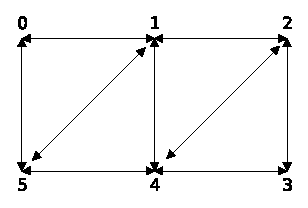
\includegraphics[bb=134 613 266 697, scale=1.4]{figs/Karcius-rede6.eps}
 % Karcius-rede6.eps: 0x0 pixel, 300dpi, 0.00x0.00 cm, bb=134 613 266 697
 \caption{Topologia F�sica da rede de 6 n�s \cite{Karcius04}.}
 \label{fig:Karcius-rede6}
\end{figure}

\begin{figure}[htb]
 \centering
 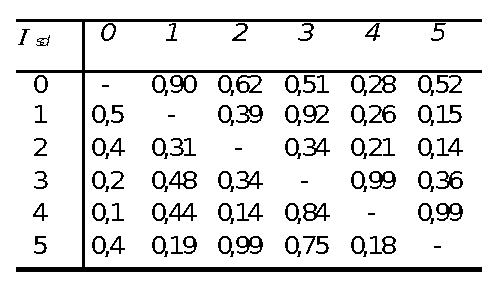
\includegraphics[bb=0 0 223 122, scale=.9]{figs/Karcius-rede6-demandas.eps}
 % Karcius-rede12-demandas.eps: 0x0 pixel, 300dpi, 0.00x0.00 cm, bb=96 243 508 387
 \caption{Matriz de demandas para a rede de 6 n�s.}
 \label{fig:Karcius-rede6-demandas}
\end{figure}

\begin{table}[!hbt]
\begin{center}
\begin{tabular}{|r|l|} \hline
Sigla  & Significado\\ \hline
$G$  & Grau L�gico\\
$L$   & Limita��o de Liga��es l�gicas das Fibras\\
$W$   & N�mero de comprimentos de onda dispon�veis\\
$S$   & N�mero de Saltos F�sicos\\
$t$   & Tempo em segundos para encontrar a primeira solu��o vi�vel\\
$Cap$ & Capacidade de Tr�fego de Cada Canal �ptico\\
$I$   & Inst�ncia Insol�vel\\ \hline
% $F$   & Tentativa Falha \\ \hline
\end{tabular}
\caption{Legendas para as Tabelas \ref{N6} e \ref{N12}.}
\label{tab:legendas-Karcius}
\end{center}
\end{table}

Os resultados para a rede de $6$ n�s est�o na Tabela \ref{N6}. Na Figura \ref{fig:Karcius-rede6} est� representada a topologia f�sica da rede de
$6$
n�s, e na Figura \ref{fig:Karcius-rede6-demandas} a matriz de demandas de tr�fego \cite{Karcius04}. A primeira coluna registra o grau l�gico de cada
inst�ncia
($G$), que neste caso foram $5$. Da segunda at� a quarta coluna ($L$, $W$ e $S$) est�o os resultados de \cite{Karcius04} e da quinta � s�tima est�o os 
resultados obtidos com a metodologia descrita nesta se��o. Note que em todas as inst�ncias foram obtidos resultados melhores para todos os par�metros.

\begin{table}[!htb]
\begin{center}
\begin{tabular}{c|ccc|ccc|ccc|} %\\ \hline
    &  \multicolumn{3}{c}{AW} \vline  & \multicolumn{6}{c}{TWA-$sl$} \\ \hline
$ G$ & $ L$ & $W$ & $ S  $ & $ L$ & $W$ & $ S $ & $ t $ & $Cap$ & $ I $\\ \hline
$ 1 $ & $ 1$ & $1$ & $ 09 $ & $ 1$ & $1$ & $ 06*$ & $00$ & $ 08$ & $ 0 $\\
$ 2 $ & $ 2$ & $2$ & $ 18 $ & $ 1$ & $1$ & $ 11*$ & $03$ & $ 03$ & $ 0 $\\
$ 3 $ & $ 2$ & $2$ & $ 32 $ & $ 1$ & $1$ & $ 14*$ & $00$ & $ 02$ & $ 0 $\\
$ 4 $ & $ 3$ & $3$ & $ 41 $ & $ 2$ & $2$ & $ 25*$ & $10$ & $ 01$ & $ 2 $\\
$ 5 $ & $ 4$ & $5$ & $ 50 $ & $ 3$ & $3$ & $ 46*$ & $00$ & $ 01$ & $ 2 $\\ \hline \hline
\end{tabular}
\caption{Resultados para a rede de $6$ n�s. * Solu��o �tima.}
\label{N6}
\end{center}
\end{table}

A oitava coluna da Tabela \ref{N6} traz o tempo, em segundos, que o SCIP levou para encontrar a primeira solu��o vi�vel ($t$). Um fato 
importante � que, em todas as inst�ncias desta bateria de testes, este tempo foi suficiente para determinar a otimalidade da solu��o vi�vel 
encontrada. Ou seja, tamb�m foi garantida a otimalidade para $S$. Essa possibilidade, al�m do interesse te�rico, evid�ncia a efici�ncia do m�todo aqui
proposto. Como base de compara��o, temos que em \cite{Karcius04} n�o � garantida a otimalidade para as m�tricas de interesse.

Ainda na Tabela \ref{N6}, na nona coluna est� a capacidade das liga��es l�gicas ($Cap$) e por fim, na �ltima coluna temos o hist�rico das tentativas 
com inst�ncia insol�vel. Nesta coluna, um $0$ (zero) significa que os resultados registrados nesta linha foram conseguidos na primeira execu��o do SCIP.
Analogamente, um n�mero diferente de zero significa a quantidade de vezes em que foram encontradas inst�ncias insol�veis, antes da execu��o que proveu o
resultado expresso nesta linha.

\begin{figure}[!htb]
 \centering
 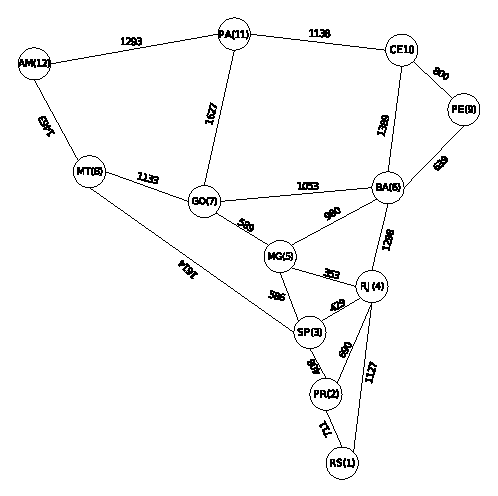
\includegraphics[bb=0 0 221 222, scale=1.4]{figs/Karcius-rede12.eps}
 % Karcius-rede6.eps: 0x0 pixel, 300dpi, 0.00x0.00 cm, bb=134 613 266 697
 \caption{Topologia F�sica da rede de 12 n�s \cite{Karcius04}}
 \label{fig:Karcius-rede12}
\end{figure}

\begin{figure}[!htb]
 \centering
 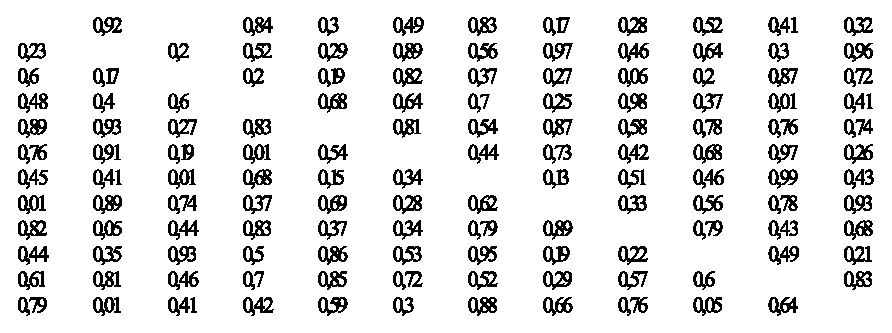
\includegraphics[bb=0 0 410 144, scale=0.9]{figs/Karcius-rede12-demandas.eps}
 % Karcius-rede12-demandas.eps: 0x0 pixel, 300dpi, 0.00x0.00 cm, bb=96 243 508 387
 \caption{Matriz de demandas para a rede de 12 n�s.}
 \label{fig:Karcius-rede12-demandas}
\end{figure}

Com o mesmo arranjo de colunas descrito acima, a Tabela \ref{N12} re�ne os resultados para a rede de $12$ n�s. Na Figura \ref{fig:Karcius-rede12} est�
representada
a topologia f�sica da rede de $6$ n�s, e na Figura \ref{fig:Karcius-rede12-demandas} sua matriz de demandas de tr�fego \cite{Karcius04}. Desta vez temos $6$
inst�ncias, do grau l�gico $1$ at� o $6$. Aqui tamb�m foram obtidos melhores resultados para o trio $L$, $W$ e $S$. Nesta etapa, os resultados de
\cite{Karcius04}
foram obtidos com $6$ horas de execu��o, enquanto os resultados com o modelo TWA levaram $7.2$ minutos para serem produzidos. 

%  \clearpage
\begin{table}[!htb]
\begin{center}
\begin{tabular}{c|ccc|ccc|ccc} %\\ \hline
    &  \multicolumn{3}{c}{AW} \vline& \multicolumn{6}{c}{TWA-$sl$} \\ \hline
$ G$ & $ L$ & $W$ & $  S  $ & $ L$ & $W$ & $  S        $ & $ t  $ & $Cap$ & $ I $\\ \hline
$ 1 $ & $ 1$ & $1$ & $ 032 $ & $ 1$ & $1$ & $ 013*      $ & $016 $ & $ 35$ & $ 0 $\\
$ 2 $ & $ 2$ & $2$ & $ 052 $ & $ 1$ & $1$ & $ 027\,\,\, $ & $031 $ & $ 10$ & $ 0 $\\
$ 3 $ & $ 3$ & $3$ & $ 078 $ & $ 2$ & $2$ & $ 066\,\,\, $ & $176 $ & $ 04$ & $ 2 $\\
$ 4 $ & $ 4$ & $4$ & $ 104 $ & $ 2$ & $2$ & $ 074\,\,\, $ & $070 $ & $ 03$ & $ 0 $\\
$ 5 $ & $ 4$ & $4$ & $ 130 $ & $ 3$ & $3$ & $ 108\,\,\, $ & $133 $ & $ 02$ & $ 2 $\\
$ 6 $ & $ 5$ & $5$ & $ 147 $ & $ 3$ & $3$ & $ 091\,\,\, $ & $003 $ & $ 02$ & $ 0 $\\ \hline \hline
\end{tabular}
\caption{Resultados para a rede de $12$ n�s. *: Solu��o �tima.}
\label{N12}
\end{center}
\end{table}

Mesmo quando n�o foi encontrado o valor �timo para  $S$, atrav�s do m�todo utilizado, a otimalidade est� garantida para os par�metros $L$
e $W$. Em particular, note que apenas a varia��o de $W$ influenciou nos resultados, pois $L$ sempre teve de ser fixado no seu valor m�ximo ($L =
W$).
Um detalhe importante � que, para a primeira inst�ncia da rede de $12$ n�s ($G=1$), o SCIP tamb�m foi capaz de provar a otimalidade
para a primeira solu��o vi�vel. Isto demonstra que o modelo TWA mant�m desempenho
aceit\'avel mesmo com uma rede de maior porte. Com esses resultados mostramos
a viabilidade do procedimento de solu��o conjunta dos problemas VTD e RWA, que � totalmente baseada no modelo apresentado neste trabalho.

\section{O Modelo KS}

Para os resultados publicados em \cite{Sivarajan01}, � feita uma modelagem MILP que minimiza congestionamento em redes sem conversores de comprimentos de
onda. Similar ao que foi feito para o TWA, em \cite{Sivarajan01} � apresentada uma forma b�sica para o modelo, com possibilidade de adapta��o para
diversos casos de uso. Descrever todas essas configura��es est� fora do escopo deste trabalho. Aqui ser� tratado apenas da particular formula��o utilizada
para produzir os resultados do exemplo pr�tico apresentados naquele artigo. Essa formula��o ser� aqui chamada de KS-$p$.

Reproduzimos nesta se��o a formula��o matem�tica para o KS-$p$. Este � um modelo de programa��o linear inteira
mista, que combina vari�veis reais e vari�veis discretas. Ele modela os quatro subproblemas do projeto de uma
WRON. Adotaremos aqui o �ndice $r$, tal como foi definido na Nota��o \ref{indice:r} (Se��o \ref{Cong}), para enumerar m�ltiplas liga��es l�gicas. A
topologia f�sica �
considerada conhecida, como para o modelo AW, sendo passada como par�metro. Al�m disso, � suposto que ela seja bidirecional e sem
multiplicidade. Os demais dados de
entrada seguem as defini��es adotadas pelo TWA, e s�o resumidos a seguir.

\begin{dados}
\label{ks:Cons}
Uma inst�ncia para o modelo KS-$p$ � definida por:
\begin{enumerate}
\item $N$ $=$ N�mero de n�s da rede.
\item $W$ $=$ M�ximo de comprimentos de onda em uma liga��o f�sica.
\item $R$ $=$ M�xima multiplicidade de liga��o l�gica.
\item $P_{sd}$ $=$ Demanda de tr�fego, com origem $s$ e destino $d$.
\item $DD_{mn}$ $=$ liga��o f�sica bidirecional entre o par $(m,n)$.
\item $GLout_v$ $=$ Grau L�gico de sa�da do n� $v$.
\item $GLin_v$ $=$ Grau L�gico de entrada do n� $v$.
\end{enumerate}
\end{dados}

\begin{vars} Vari�veis do modelo KS-$p$:
\label{ks:vars}
\begin{enumerate}
\item $b_{ijr} \in \{0,1\}$, indica a exist�ncia ($1$) ou n�o ($0$) da liga��o l�gica $(i,j)$ de �ndice $r$.

\item  $C_{ij}^{wr} \in \{0,1\}$, indica se $b_{ijr}$ usa o comprimento de onda $w$.

\item  $C_{mnij}^{wr} \in \{0,1\}$, indica se $C_{ij}^{wr}$ passa pela liga��o f�sica $(m,n)$.

\item  $\lambda_{ijr}^{s}\in \mathbb{R^+}$, � quantidade de tr�fego fluindo de uma fonte $s$ passando por $b_{ijr}$.

\item  $\lambda_{ijr}\in \mathbb{R^+}$, tr�fego total em $b_{ijr}$.

\item  $\lambda_{max} \in \mathbb{R^+}$, congestionamento da rede.

\end{enumerate}
\end{vars}

\textbf{Fun��o Objetivo}
\begin{itemize}

\item Minimize o Congestionamento:
\begin{equation}
\lambda_{max}
\label{ks:fo:hmax}
\end{equation}

\end{itemize}

\textbf{Restri��es}

\begin{itemize}

\item Distribui��o do tr�fego:

\begin{equation}
 \lambda_{ijr}^{s}  \leqslant b_{ijr}\cdot A_s \Forall{(i,j,r,s)}
\label{ks:rest:DistTraf}
\end{equation}

\item Rotas F�sicas

\begin{equation}
 C_{mnij}^{wr} \leqslant C_{ij}^{wr} \Forall{(i,j,w,r,m,n)}
\label{ks:rest:Rotas1}
\end{equation}

\begin{equation}
 \sum_{ijr} C_{mnij}^{wr} \leqslant 1 \Forall{(w,m,n)}
\label{ks:rest:Rotas2}
\end{equation}

\item Aloca��o de Comprimento de Onda:

\begin{equation}
 \sum_w C_{ij}^{wr} = b_{ijr} \Forall{(i,j,r)}
\label{ks:rest:W}
\end{equation}

\item Conserva��o das Rotas sobre a Topologia F�sica:

\begin{equation}
 \forall \,  \mbox{\small$(i,j,r,n)$}, \quad \sum_{mw} C_{mnij}^{wr}\cdot D_{mn} - \sum_{mw} C_{nmij}^{wr}\cdot D_{nm} = 
  \left\{\begin{aligned} b_{ijr}, & \quad n=j\\
								-b_{ijr}, & \quad n=i\\
								0, & \quad \text{caso contr�rio} \end{aligned}\right.
\label{ks:rest:Fis}
\end{equation}

\item Conserva��o de Fluxo:

\begin{equation}
 \forall \,  \mbox{\small$(s,i)$}, \quad \sum_{jr} \lambda_{ijr}^{s} - \sum_{jr} \lambda_{jir}^{s} = \left\{\begin{aligned} A_s, & \quad s=i\\
						  -P_{si}, & \quad \text{caso contr�rio} \end{aligned}\right.
\label{ks:rest:Flow}
\end{equation}

\item Congestionamento:

\begin{equation}
 \lambda_{ijr} = \sum_{s} \lambda_{ijr}^{s} \Forall{(i,j,r)}
\label{ks:rest:hmax1}
\end{equation}

\begin{equation}
 \lambda_{ijr} \leqslant \lambda_{max} \Forall{(i,j,r)}
\label{ks:rest:hmax2}
\end{equation}

\item Grau l�gico:

\begin{equation}
\sum_{jr}  b_{ijr}  = GLout_i \Forall{i}
\label{ks:rest:gl1}
\end{equation}

\begin{equation}
\sum_{ir}  b_{ijr}  = GLin_j \Forall{j}
\label{ks:rest:gl2}
\end{equation}

\end{itemize}

\subsection{Compara��o entre os Modelos KS-$p$ e TWA}

Apesar de fazer a distribui��o do tr�fego de forma agregada, no modelo KS-$p$ essa t�cnica n�o foi aplicada ao roteamento de comprimentos de onda.
Semelhante ao modelo AW, s�o definidas tr�s vari�veis diferentes para as liga��es l�gicas, roteamento e aloca��o de comprimentos de onda. Mas no
modelo KS-$p$, conseguiu-se uma modelagem mais concisa, em compara��o com o AW, ainda sem possuir as limita��es presentes no TWA. Ele possui as mesmas
vantagens que o AW em rela��o ao TWA, pois a distribui��o do tr�fego e configura��o da rotas s�o expl�citas. 

Em rela��o ao AW, o modelo KS-$p$ ainda tem a
vantagem de permitir multiplicidade de liga��es l�gicas. Todavia, n�o foi prevista em \cite{Sivarajan01} a possibilidade da topologia f�sica ser uma das
vari�veis do problema. O artigo indica como poderia ser adicionado suporte � multiplicidade de liga��es f�sicas, modificando o modelo b�sico KS, mas seria
necess�rio modicar e adicionar, tanto restri��es quanto vari�veis. 

O relacionamento entre a topologia f�sica e as rotas f�sicas � feito sob um diferente ponto de vista no TWA. No modelo KS-$p$, � a Restri��o
\ref{rest:DefFis} quem cuida da conserva��o da rotas f�sicas, construindo caminhos sobre a topologia f�sica. No TWA, a conserva��o dos percursos � feita
separadamente (Restri��o \ref{rest:DefCapFlow}), dando mais autonomia aos componentes topol�gicos. Pois eles � que defini��o a topologia f�sica (Se��o
\ref{cap:twa-sec:Fis}), se esta � vari�vel, ou ser�o apenas limitados por ela pontualmente (Se��o \ref{cap:cases-sec:fis}). Ao combinar a adequa��o �
topologia f�sica e a conserva��o de rotas em uma mesma restri��o (Restri��o \ref{ks:rest:Fis}), o modelo KS-$p$ n�o permite considerar a topologia f�sica
como vari�vel, sem deixar de ser linear. Na rela��o a seguir s�o comparados paralelamente os modelos KS-$p$ e TWA, em termos de
funcionalidade.

\begin{itemize}
	\item As vari�veis de \ref{ks:vars}.1 a \ref{ks:vars}.3 correspondem ao componente topol�gico do TWA, definido na Vari�vel \ref{twa:var:B};
	\item A vari�vel \ref{ks:vars}.4 corresponde � fra��o de tr�fego agregado, Vari�vel \ref{FlowVar};
	\item As Restri��es de \ref{ks:rest:DistTraf} a \ref{ks:rest:Fis} correspondem a Restri��o \ref{rest:DefCapFlow}, de continuidade de comprimentos de
	onda, mas aqui a topologia f�sica � envolvida na conserva��o dos percursos;
	\item A Restri��o \ref{ks:rest:Fis} se assemelha a Restri��o \ref{rest:DefFis}, de controle da topologia f�sica, no
sentido de limita��o dos componentes topol�gicos, como foi comentado na Se��o \ref{cap:cases-sec:fis};
	\item A Restri��o \ref{ks:rest:Flow} corresponde as restri��es de conserva��o de fluxo \ref{rest:ConservFlowOut} e \ref{rest:ConservFlow};
	\item O controle do congestionamento e grau l�gico equivale ao que foi feito nas Se��es \ref{Cong} e \ref{ConservGl}, respectivamente;
% 	\item O controle do n�mero de liga��es l�gicas em cada liga��o f�sica equivale ao que foi feito na Se��o \ref{LimW};
% 	\item O controle do n�mero de saltos f�sicos equivale ao que foi feito na Se��o \ref{cap:cases-sec:LimB};
\end{itemize}

Na tabela \ref{tab:ks:num_var} est�o resumidos os dados a cerca do n�mero de vari�veis bin�rias, de vari�veis reais e do n�mero equa��es no modelo KS-$p$.
Eles s�o apresentados em nota��o assint�tica e em valores absolutos. Para fins de compara��o, vale relembrar neste ponto que o modelo KS-$p$ n�o suporta
multiplicidade de liga��es f�sicas, al�m de considerar a topologia f�sica como um dado de entrada. O fator $R$, m�xima multiplicidade de uma liga��o
l�gica, apenas influencia na contagem de vari�veis e equa��es do TWA no contexto da Se��o \ref{cap:cases-sec:CongMulti}, para minimiza��o do
congestionamento sem perda de multiplicidade de liga��es l�gicas.
 
\begin{table}[htb]
{%
\newcommand{\mc}[3]{\multicolumn{#1}{#2}{#3}}
\begin{center}
\begin{tabular}{llll}\hline
\mc{1}{|c|}{M�trica} & \mc{1}{c|}{Equa��es} & \mc{1}{l|}{Reais} & \mc{1}{|l|}{Bin�rias}\\\hline
\mc{1}{|l|}{Custo Assint�tico} & \mc{1}{|l|}{$\Theta(N^4WR)$} & \mc{1}{|l|}{$\Theta(N^3R)$} & \mc{1}{|l|}{$\Theta(N^4WR)$}\\\hline
\mc{1}{|l|}{Valores Absolutos} & \mc{1}{|l|}{$N^4WR\!+\!2N^3R\!+\!N^2(W\!+\!3R)\!+\!2N$} &
\mc{1}{|l|}{$N^3R\!+\!N^2R$} & \mc{1}{|l|}{$N^4WR\!+\!N^2RW$}\\\hline
\end{tabular}
\end{center}
}%
\caption{Numero de vari�veis bin�rias, reais e equa��es no modelo KS-$p$.}
\label{tab:ks:num_var}
\end{table}

\subsection{Metodologia Baseada no Modelo KS-$p$}

Em \cite{Sivarajan01} foram feitos testes para uma rede de $14$ n�s, a mesma que ser� estuda na se��o seguinte \cite{ram96}. Segundo os autores, a
formula��o KS-$p$ n�o � computacionalmente trat�vel para este caso, o que justificou a proposi��o de um m�todo heur�stico. Ele consiste na aplica��o da
heur�stica LPLDA \cite{ram96}, seguida de dois algoritmos de arredondamento, finalizando com um algoritmo de colora��o de grafos \cite{cormen02}.
Introduzida em \cite{ram96}, mesmo trabalho de origem da HLDA, a heur�stica LPLDA � baseada em um m�todo iterativo para constru��o de limitantes inferiores
para o congestionamento (ILB - \textit{Iterative Lower Bound}), descrito a seguir. 

O ILB consiste em substituir a Restri��o \ref{ks:rest:hmax2} do modelo KS-$p$ por \ref{ks:rest:hmaxLB},
onde $\lambda_{max}^{LB_0}$ � qualquer limitante inferior (LB) para $\lambda_{max}$, podendo ser zero. Em seguida s�o relaxadas as vari�veis inteiras,
permitindo assumir qualquer valor entre o m�ximo e o m�nimo de seu dom�nio. Por exemplo, uma vari�vel bin�ria tem dom�nio $\{ 0, 1 \}$, relaxando-a da forma
indicada ela poder� assumir qualquer valor real entre $0$ e $1$. Deste modo, o modelo MILP se torna um LP (\textit{linear problem}). A Restri��o
\ref{ks:rest:hmaxLB} n�o influencia no modelo MILP, mas no relaxado sim, for�ando que o �timo da vers�o LP seja maior ou igual � $\lambda_{max}^{LB_0}$.
Como o �timo de uma vers�o relaxada � menor ou igual ao �timo do modelo de minimiza��o original \cite{beas}, segue que o �timo da vers�o relaxada � tamb�m
um limitante inferior para $\lambda_{max}$. Assim, denotando o �timo do modelo relaxado por $\lambda_{max}^{LB_1}$ e substituindo $\lambda_{max}^{LB_0}$ por
ele em \ref{ks:rest:hmaxLB}, ser� produzido um novo LB, que pode ser chamado de $\lambda_{max}^{LB_2}$. Deste modo, iterativamente pode-se ir melhorando o
LB original, o que constitui o m�todo interativo.

\textbf{Restri��o}
\begin{itemize}
\item Plano de Corte para o Congestionamento:
\begin{equation}
  \lambda_{max} \geqslant \lambda_{ijr} + \lambda_{max}^{LB_0}\cdot(1 - b_{ijr}) \Forall{(i,j,r)}
\label{ks:rest:hmaxLB}
\end{equation}
\end{itemize}

O LPLDA consiste de aplicar um algoritmo de arredondamento �s liga��es l�gicas ($b_{ijr}$), na solu��o da �ltima itera��o do ILB. Este � iterado $25$
vezes, valor suficiente para se convergir o LB satisfatoriamente, conforme foi determinado em \cite{ram96}.
Resumidamente, as
vari�veis relaxadas s�o ordenadas pelo valor obtido para cada uma. Ent�o, seguindo essa ordena��o, elas s�o arredondadas para os valores inteiros mais
pr�ximos, preservando grau l�gico. Determinada a topologia l�gica, o tr�fego � roteado utilizando somente as restri��es relacionadas ao tr�fego no MILP:
Restri��es de \ref{ks:rest:Flow} a \ref{ks:rest:hmax2}, mas a Restri��o \ref{ks:rest:DistTraf}.

Ap�s aplicar o LPLDA, s�o utilizados outros dois algoritmos de
arredondamento, similares ao que � usado no LPLDA, mas aplicados �s vari�veis $C_{ij}^{wr}$ e $C_{mnij}^{wr}$, nessa ordem. Para as vari�veis $C_{ij}^{wr}$,
para cada $b_{ijr} = 1$, o algoritmo arredonda para $1$ a maior delas anulando as demais. Assim � associado o comprimento de onda � liga��o l�gica
$b_{ijr}$. As vari�veis $C_{mnij}^{wr}$, para cada $C_{ij}^{wr} = 1$, s�o arredondadas para $1$ se formam um caminho que atenda � $C_{ij}^{wr}$,
anulando as demais. O caminho � constru�do a partir de $i$, sempre pegando a vari�vel $C_{mnij}^{wr}$ de maior valor.

Os algoritmos utilizados para arredondar as vari�veis $C_{ij}^{wr}$ e $C_{mnij}^{wr}$, n�o verificam se h� duas rotas f�sicas utilizando o mesmo
comprimento de onda em uma determinada liga��o f�sica. Essa situa��o � chamada de colis�o de comprimentos de onda (\textit{wavelength clash}). Para corrigir
poss�veis colis�es, o m�todo utilizado em \cite{Sivarajan01} � finalizado com a aplica��o de uma algoritmo de colora��o de grafos de caminhos
\cite{beas}, que refaz a aloca��o de comprimentos de onda. Maiores detalhes sobre este �ltimo algoritmo podem ser vistos em \cite{Sivarajan06}, dos mesmos
autores. 

Nos resultados que foram produzidos, a topologia f�sica e a matriz de demandas utilizadas s�o da rede de $14$ n�s tamb�m utilizada em \cite{ram96}. Como
para o modelo AW, as inst�ncias neste caso tamb�m s�o definidas pelo grau l�gico $G$. Para definir uma inst�ncia do modelo KS-$p$, resta definir $W$ e $R$.
Para os resultados produzidos em \cite{Sivarajan01}, n�o foi utilizada multiplicidade de liga��es logicas, ou seja, $R = 1$. 

Para aplicar o ILB, dependendo
do valor de $W$, o modelo relaxado pode n�o ser resol�vel. � ent�o � determinado o valor m�nimo de $W$, de modo que o modelo relaxado n�o seja insol�vel,
realizando no conjunto de poss�veis valores de $W$ uma busca bin�ria \cite{cormen02}, com n�mero de passos logar�tmico. Sendo que o menor valor poss�vel
para $W$ � $1$ (sem multiplexa��o) e o valor m�ximo � $N^2 - N$, o n�mero de combina��es $(i,j)$ poss�veis, sem multiplicidade. Onde cada liga��o
l�gica teria seu pr�prio comprimento de onda. Essa busca bin�ria � feita testando os valores de $W$ no modelo relaxado. Estabelecido o $W$ m�nimo para
determinado $G$, nos graus l�gicos superiores os m�nimos s�o maiores ou iguais a esse, como foi comentado na Se��o \ref{cap:testes-sec:karcius}.
Portanto, realizando os testes do menor grau l�gico para o maior, a busca pelo $W$ m�nimo n�o � refeita do in�cio.

Na fase final deste m�todo, quando a aloca��o de comprimentos de onda � refeita, o algoritmo de colora��o de grafos de caminhos n�o � impedido de
ultrapassar o $W$ minimo, estabelecido acima. Todo o procedimento � resumido a seguir:

\begin{enumerate}
	\item Encontra o $W$ m�nimo para o $G$ atual;
	\item Executa $25$ itera��es do ILB;
	\item Arredonda os maiores $b_{ijr}$ para $1$ e os menores para $0$, preservando grau l�gico;
	\item Distribui o tr�fego na topologia l�gica, obtendo o congestionamento;
	\item Arredonda os maiores $C_{ij}^{wr}$ para $1$ se $b_{ijr} = 1$, e o restante para $0$;
	\item Arredonda para $1$ o caminho com os maiores $C_{mnij}^{wr}$, para cada $C_{ij}^{wr} = 1$, anulando os demais;
	\item Refaz a aloca��o de comprimentos de onda, com possibilidade de ultrapassar o $W$ m�nimo;
\end{enumerate}

Nos resultados para a modelagem KS-$p$, cada otimiza��o do modelo relaxado levou em m�dia $5$ minutos. Al�m das $25$ itera��es do ILB, o modelo
relaxado tamb�m foi usado para determinar o $W$ m�nimo em cada inst�ncia. As heur�sticas aplicadas subsequentemente ao ILB levaram menos de um minuto para
cada inst�ncia. A otimalidade, quanto ao congestionamento, s� p�de ser garantida nesses resultados quando o valor vi�vel encontrado era igual ao
\textit{lower bound} obtido. Esses resultados foram produzidos com a \textit{IBM's Optimization Subroutine Library (OSL)} em um computador IBM 43P/RS6000.


\section{Compara��o de Resultados com o modelo KS}
\label{cap:testes-sec:sivarajan}

 Nos resultados que iremos confrontar, � considerado o grau l�gico da rede ($G$), n�o h� multiplicidade de liga��es l�gicas e a fun��o objetivo � o
congestionamento. Para produzir resultados pass�veis de compara��o, s�o acrescentadas � modelagem b�sica do TWA, mostrada na Se��o \ref{Basic}: as Restri��es
\ref{ConservGl} de controle do grau l�gico; a Restri��o \ref{cases:rest:Ml} de controle de multiplicidade de liga��es l�gicas, com $M=1$; e a Restri��o
\ref{Hmax} que determina o congestionamento como fun��o objetivo. Esta formula��o espec�fica � denominada de
TWA$c_1$.

O computador onde foram executados os experimentos desta se��o possui a seguinte configura��o: 
\textit{desktop} \textit{PC};
executando o sistema operacional \textit{GNU/Linux Kubuntu}, vers�o $ 9.04$ $32 bits$;
equipada com processador \textit{Intel Pentium\rr $4$} $3.00GHz$ de $2$ n�cleos, com $2048 KB$ de \textit{cache} e $1.5GB$ de RAM.
 
\begin{figure}[htb]
 \centering
 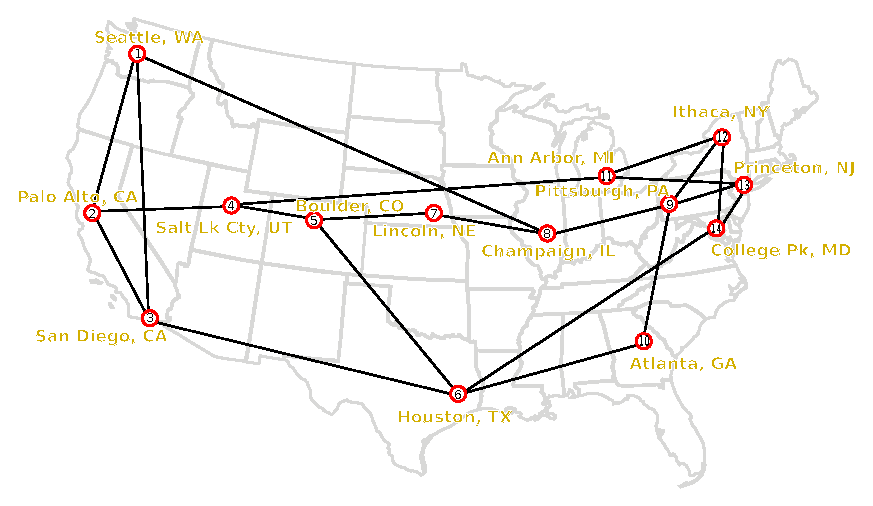
\includegraphics[bb=115 313 518 540, scale=1.12]{figs/nsfnet_14nodes.eps}
 % nsfnet.eps: 0x0 pixel, 300dpi, 0.00x0.00 cm, bb=115 313 518 540
 \caption{Rede de 14 n�s NSFNET \cite{Sivarajan01}.}
 \label{fig:nsfnet}
\end{figure}

\begin{figure}[htb]
	\centering
	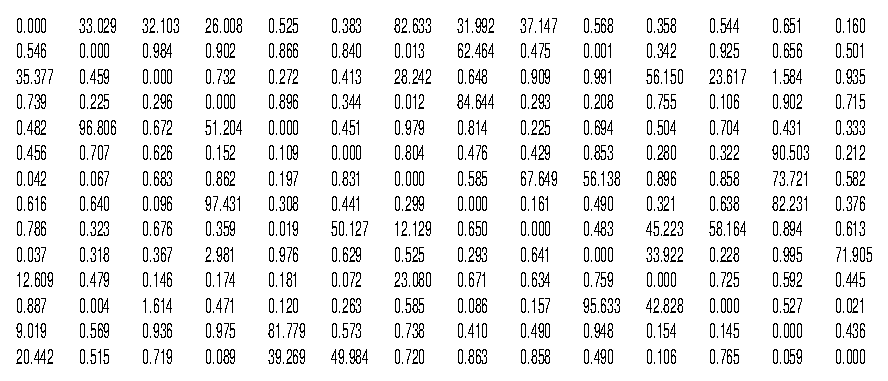
\includegraphics[bb=0 0 410 167,scale=1.1]{./figs/p1.eps}
	% p1.eps: 0x0 pixel, 300dpi, 0.00x0.00 cm, bb=0 0 410 167
	\caption{Matriz de demandas $P1$ \cite{ram96}.}%\hline
	\label{fig:p1}
\end{figure}

\begin{figure}[htb]
	\centering
	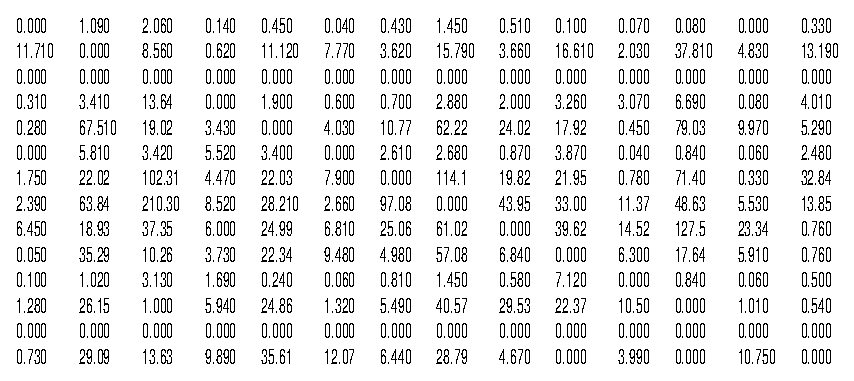
\includegraphics[bb=0 0 394 167,scale=1.1]{./figs/p2.eps}
	% p2.eps: 0x0 pixel, 300dpi, 0.00x0.00 cm, bb=0 0 394 167
	\caption{Matriz de demandas $P2$ \cite{ram96}.}
	\label{fig:p2}
\end{figure}

% \begin{table}[htb]
%  \centering
% \caption{Matriz de demandas $P1$ \cite{ram96}.}
% % \scriptsize
% % \rmfamily
% % \ttfamily
% \bfseries
% \sffamily
% \tiny
% \begin{tabular}{llllllllllllll} %\hline
% 	0.000 & 33.029 & 32.103 & 26.008 & 0.525 & 0.383 & 82.633 & 31.992 & 37.147 & 0.568 & 0.358 & 0.544 & 0.651 & 0.160\\
% 	0.546 & 0.000 & 0.984 & 0.902 & 0.866 & 0.840 & 0.013 & 62.464 & 0.475 & 0.001 & 0.342 & 0.925 & 0.656 & 0.501\\
% 	35.377 & 0.459 & 0.000 & 0.732 & 0.272 & 0.413 & 28.242 & 0.648 & 0.909 & 0.991 & 56.150 & 23.617 & 1.584 & 0.935\\
% 	0.739 & 0.225 & 0.296 & 0.000 & 0.896 & 0.344 & 0.012 & 84.644 & 0.293 & 0.208 & 0.755 & 0.106 & 0.902 & 0.715\\
% 	0.482 & 96.806 & 0.672 & 51.204 & 0.000 & 0.451 & 0.979 & 0.814 & 0.225 & 0.694 & 0.504 & 0.704 & 0.431 & 0.333\\
% 	0.456 & 0.707 & 0.626 & 0.152 & 0.109 & 0.000 & 0.804 & 0.476 & 0.429 & 0.853 & 0.280 & 0.322 & 90.503 & 0.212\\
% 	0.042 & 0.067 & 0.683 & 0.862 & 0.197 & 0.831 & 0.000 & 0.585 & 67.649 & 56.138 & 0.896 & 0.858 & 73.721 & 0.582\\
% 	0.616 & 0.640 & 0.096 & 97.431 & 0.308 & 0.441 & 0.299 & 0.000 & 0.161 & 0.490 & 0.321 & 0.638 & 82.231 & 0.376\\
% 	0.786 & 0.323 & 0.676 & 0.359 & 0.019 & 50.127 & 12.129 & 0.650 & 0.000 & 0.483 & 45.223 & 58.164 & 0.894 & 0.613\\
% 	0.037 & 0.318 & 0.367 & 2.981 & 0.976 & 0.629 & 0.525 & 0.293 & 0.641 & 0.000 & 33.922 & 0.228 & 0.995 & 71.905\\
% 	12.609 & 0.479 & 0.146 & 0.174 & 0.181 & 0.072 & 23.080 & 0.671 & 0.634 & 0.759 & 0.000 & 0.725 & 0.592 & 0.445\\
% 	0.887 & 0.004 & 1.614 & 0.471 & 0.120 & 0.263 & 0.585 & 0.086 & 0.157 & 95.633 & 42.828 & 0.000 & 0.527 & 0.021\\
% 	9.019 & 0.569 & 0.936 & 0.975 & 81.779 & 0.573 & 0.738 & 0.410 & 0.490 & 0.948 & 0.154 & 0.145 & 0.000 & 0.436\\
% 	20.442 & 0.515 & 0.719 & 0.089 & 39.269 & 49.984 & 0.720 & 0.863 & 0.858 & 0.490 & 0.106 & 0.765 & 0.059 & 0.000\\
% \end{tabular}
% \label{tab:p1-demandas}
% \end{table}

% \begin{table}[htb]
% \caption{Matriz de demandas $P2$ \cite{ram96}.}
%  \centering
% \bfseries
% \sffamily
% \tiny
% \begin{tabular}{llllllllllllll} %\hline
% 0.000 & 1.090 & 2.060 & 0.140 & 0.450 & 0.040 & 0.430 & 1.450 & 0.510 & 0.100 & 0.070 & 0.080 & 0.000 & 0.330\\
% 11.710 & 0.000 & 8.560 & 0.620 & 11.120 & 7.770 & 3.620 & 15.790 & 3.660 & 16.610 & 2.030 & 37.810 & 4.830 & 13.190\\
% 0.000 & 0.000 & 0.000 & 0.000 & 0.000 & 0.000 & 0.000 & 0.000 & 0.000 & 0.000 & 0.000 & 0.000 & 0.000 & 0.000\\
% 0.310 & 3.410 & 13.64 & 0.000 & 1.900 & 0.600 & 0.700 & 2.880 & 2.000 & 3.260 & 3.070 & 6.690 & 0.080 & 4.010\\
% 0.280 & 67.510 & 19.02 & 3.430 & 0.000 & 4.030 & 10.77 & 62.22 & 24.02 & 17.92 & 0.450 & 79.03 & 9.970 & 5.290\\
% 0.000 & 5.810 & 3.420 & 5.520 & 3.400 & 0.000 & 2.610 & 2.680 & 0.870 & 3.870 & 0.040 & 0.840 & 0.060 & 2.480\\
% 1.750 & 22.02 & 102.31 & 4.470 & 22.03 & 7.900 & 0.000 & 114.1 & 19.82 & 21.95 & 0.780 & 71.40 & 0.330 & 32.84\\
% 2.390 & 63.84 & 210.30 & 8.520 & 28.210 & 2.660 & 97.08 & 0.000 & 43.95 & 33.00 & 11.37 & 48.63 & 5.530 & 13.85\\
% 6.450 & 18.93 & 37.35 & 6.000 & 24.99 & 6.810 & 25.06 & 61.02 & 0.000 & 39.62 & 14.52 & 127.5 & 23.34 & 0.760\\
% 0.050 & 35.29 & 10.26 & 3.730 & 22.34 & 9.480 & 4.980 & 57.08 & 6.840 & 0.000 & 6.300 & 17.64 & 5.910 & 0.760\\
% 0.100 & 1.020 & 3.130 & 1.690 & 0.240 & 0.060 & 0.810 & 1.450 & 0.580 & 7.120 & 0.000 & 0.840 & 0.060 & 0.500\\
% 1.280 & 26.15 & 1.000 & 5.940 & 24.86 & 1.320 & 5.490 & 40.57 & 29.53 & 22.37 & 10.50 & 0.000 & 1.010 & 0.540\\
% 0.000 & 0.000 & 0.000 & 0.000 & 0.000 & 0.000 & 0.000 & 0.000 & 0.000 & 0.000 & 0.000 & 0.000 & 0.000 & 0.000\\
% 0.730 & 29.09 & 13.63 & 9.890 & 35.61 & 12.07 & 6.440 & 28.79 & 4.670 & 0.000 & 3.990 & 0.000 & 10.750 & 0.000\\
% \end{tabular}
% \label{tab:p2-demandas}
% \end{table}


\begin{table}[htb]
\caption{Matriz de dist�ncias para a NSFNET, em centenas de milhas.}
 \centering
% \tiny
\begin{tabular}{llllllllllllll} \hline
0	&	7	&	10	&	7	&	10	&	19	&	13	&	16	&	21	&	21	&	19	&	22	&	24	&	22\\
7	&	0	&	4	&	5	&	9	&	16	&	14	&	18	&	22	&	21	&	20	&	24	&	25	&	21\\
10	&	4	&	0	&	6	&	8	&	12	&	13	&	17	&	21	&	19	&	19	&	23	&	24	&	19\\
7	&	5	&	6	&	0	&	4	&	12	&	8	&	12	&	17	&	16	&	13	&	18	&	19	&	16\\
10	&	9	&	8	&	4	&	0	&	8	&	4	&	9	&	13	&	12	&	11	&	15	&	16	&	12\\
19	&	16	&	12	&	12	&	8	&	0	&	8	&	8	&	11	&	7	&	11	&	14	&	14	&	12\\
13	&	14	&	13	&	8	&	4	&	8	&	0	&	5	&	9	&	8	&	7	&	10	&	11	&	8\\
16	&	18	&	17	&	12	&	9	&	8	&	5	&	0	&	5	&	5	&	3	&	6	&	7	&	5\\
21	&	22	&	21	&	17	&	13	&	11	&	9	&	5	&	0	&	5	&	2	&	2	&	2	&	5\\
21	&	21	&	19	&	16	&	12	&	7	&	8	&	5	&	5	&	0	&	6	&	7	&	7	&	6\\
19	&	20	&	19	&	13	&	11	&	11	&	7	&	3	&	2	&	6	&	0	&	4	&	5	&	6\\
22	&	24	&	23	&	18	&	15	&	14	&	10	&	6	&	2	&	7	&	4	&	0	&	2	&	5\\
24	&	25	&	24	&	19	&	16	&	14	&	11	&	7	&	2	&	7	&	5	&	2	&	0	&	1\\
22	&	21	&	19	&	16	&	12	&	12	&	8	&	5	&	5	&	6	&	6	&	5	&	1	&	0\\
\end{tabular}
\label{tab:distancias-NSFNET}
\end{table}

Na Figura \ref{fig:nsfnet} est� representada a topologia f�sica da rede NSFNET, na qual s�o baseados os testes em \cite{Sivarajan01}. Nas Tabelas
\ref{fig:p1} e \ref{fig:p2}, respectivamente, est�o as matrizes de demandas $P1$ e $P2$ da NSFNET \cite{ram02}. J� na Tabela
\ref{tab:distancias-NSFNET} est�o as dist�ncias entre os n�s da topologia f�sica da NSFNET adotada, em centenas de milhas.

\begin{table}
% [!ht]
\begin{center}
\caption{Legendas para as Tabelas \ref{p1} e \ref{p2}.}

\begin{tabular}{|r|l|} \hline
Sigla  & Significado\\ \hline
$G$  & Grau L�gico\\
$W$   & N�mero de comprimentos de onda dispon�veis\\
MTB  & \textit{Minimum Trafic Bound}\\
MILP & Resultados obtidos pelo SCIP\\
$T$   & Tempo em minutos gasto com o SCIP\\
KS & Melhores resultados com o modelo KS\\
$LB$   & Lower Bound para o congestionamento\\
$UB$   & Uper Bound para o congestionamento\\ \hline
\end{tabular}
\label{tab:legendas-Sivarajan}
 \end{center}
\end{table}

\begin{table}
% [!ht]
 \begin{center}
\caption{Resultados para a matriz $P1$. *: �timo alcan�ado.}
\begin{tabular}{|c|crrr|rrc|}
\hline $P1$ &    \multicolumn{4}{|c|}{TWA$c_1$}     & \multicolumn{3}{c|}{KS}   \\ \hline \hline
		  $G$ & $W$ & $T_{(m)}$ &   MTB    &   MILP   & $LB$     & $UB$     & $W$ \\ \hline
		  $ 2$ & $2$ & $451$     & $126.87$ & $143.66$ & $126.74$ & $145.74$ & $4$ \\ \hline
		  $ 3$ & $3$ & $221$     & $ 84.58$ & $^*84.58$& $84.58$  & $^*84.58$& $4$ \\ \hline
		  $ 4$ & $3$ & $8$       & $ 63.44$ & $69.17$  & $63.43$  & $70.02$  & $4$ \\ \hline
		  $ 5$ & $4$ & $225$     & $ 50.75$ & $50.82$  & $50.74$  & $50.94$  & $5$ \\ \hline
		  $ 6$ & $4$ & $24$      & $ 42.29$ & $43.54$  & $42.29$  & $44.39$  & $6$ \\ \hline
		  $ 7$ & $5$ & $65$      & $ 36.25$ & $^*36.25$& $36.25$  & $36.43$  & $6$ \\ \hline
		  $ 8$ & $6$ & $102$     & $ 31.72$ & $^*31.72$& $31.72$  & $31.77$  & $7$ \\ \hline
		  $ 9$ & $7$ & $131$     & $ 28.19$ & $^*28.19$& $28.19$  & $28.37$  & $9$ \\ \hline
		  $10$ & $8$ & $72$      & $ 25.37$ & $25.53$  & $25.37$  & $25.64$  & $9$ \\ \hline
		  $11$ & $9$ & $200$     & $ 23.07$ & $23.31$  & $23.00$  & $23.08$  & $11$\\ \hline
		  $12$ & $11$& $140$     & $ 21.14$ & $21.35$  & $21.27$  & $21.39$  & $12$\\ \hline
		  $13$ & $13$& $16$      & $ 19.52$ & $^*20.25$& $20.24$  & $20.25$  & $13$\\ \hline
\end{tabular}                                               
\label{p1}                                                  
 \end{center}                                              
\end{table}                                                 
                                                                                                                                                                  
                                                                                                                                                                  
                                                                                                                                                        
% \newpage
\begin{table}
% [!ht]
 \begin{center}
\caption{Resultados para a matriz $P2$. *: �timo alcan�ado.}
\begin{tabular}{|c|crrr|rrc|}
\hline $P2$ &    \multicolumn{4}{|c|}{TWA$c_1$}     & \multicolumn{3}{c|}{KS}       \\ \hline \hline
		  $G$ & $W$ & $T_{(m)}$ &   MTB    &    MILP    & $LB$     & $UB$      & $W$  \\ \hline
		  $ 2$ & $1$ & $152$     & $284.66$ & $^*292.31$ & $284.26$ & $389.93$  & $2$  \\ \hline
		  $ 3$ & $2$ & $4.4$     & $189.78$ & $^*189.78$ & $189.76$ & $217.80$  & $4$  \\ \hline
		  $ 4$ & $2$ & $2$       & $142.33$ & $^*142.33$ & $142.33$ & $152.99$  & $3$  \\ \hline
		  $ 5$ & $3$ & $4$       & $113.87$ & $^*113.87$ & $113.87$ & $^*113.87$& $4$  \\ \hline
		  $ 6$ & $3$ & $3.9$     & $94.89$  & $^*94.89$  & $94.89$  & $^*94.89$ & $5$  \\ \hline
		  $ 7$ & $4$ & $4.3$     & $81.33$  & $^*81.33$  & $81.33$  & $^*81.33$ & $6$  \\ \hline
		  $ 8$ & $4$ & $6.8$     & $71.17$  & $^*71.17$  & $71.17$  & $^*71.17$ & $6$  \\ \hline
		  $ 9$ & $5$ & $20.9$    & $63.26$  & $^*63.26$  & $62.15$  & $63.26$   & $9$  \\ \hline
		  $10$ & $6$ & $20.1$    & $56.93$  & $^*56.93$  & $56.93$  & $^*56.93$ & $10$ \\ \hline
		  $11$ & $6$ & $23.2$    & $51.75$  & $^*51.75$  & $51.75$  & $^*51.75$ & $10$ \\ \hline
		  $12$ & $7$ & $23.1$    & $47.44$  & $^*47.44$  & $47.44$  & $^*47.44$ & $13$ \\ \hline
		  $13$ & $7$ & $14.8$    & $43.79$  & $^*43.79$  & $43.79$  & $^*43.79$ & $13$ \\ \hline
\end{tabular}
\label{p2}
 \end{center}
\end{table}
% \clearpage

Nas Tabelas \ref{p1} e \ref{p2} s�o confrontados os resultados obtidos com o TWA$c_1$ e os encontrados em \cite{Sivarajan01}, com o modelo KS. Para cada
grau
l�gico, s�o exibidos: na coluna MILP, o valor de congestionamento obtido executando o modelo MILP do TWA$c_1$ com o SCIP; na coluna $T$, o tempo gasto
pelo SCIP para chegar a essa solu��o; na coluna $W$, o n�mero de comprimentos de onda utilizados pelo TWA$c_1$; e na coluna MTB, o \textit{Minimum Trafic
Bound}
para cada inst�ncia. Tamb�m s�o exibidos, para o modelo KS, na coluna $UB$, as melhores solu��es para o congestionamento encontradas em  \cite{Sivarajan01},
e nas
colunas $LB$ e $W$, os respectivos \textit{lower bounds} e  n�mero de comprimentos de onda utilizados pelo KS. Quando o valor de congestionamento
corresponde ao
�timo da inst�ncia, ele � marcado com um asterisco.

Para ambas as matrizes, foram obtidos melhores resultados com o TWA$c_1$, em compara��o com os resultados para o modelo KS, tanto para o valor de
congestionamento quanto para o n�mero de comprimentos de onda utilizados. Outro fato importante � qualidade alcan�ada pelo MTB em todas as inst�ncias,
praticamente igual ao \textit{lower bound} obtido em \cite{Sivarajan01}, mas com demanda de tempo desprez�vel. Esse � um resultado expressivo, frente aos $125$
minutos, em m�dia, gastos com o m�todo iterativo \cite{ram02}. Em $62\%$ das inst�ncias, o MTB equivale ao �timo. E mesmo quando o �timo diferiu do MTB, no pior
caso, o MTB ficou menos de $5\%$ abaixo do �timo. Por fim vale ressaltar que foram obtidas solu��es �timas para $70\%$ das inst�ncias com o TWA$c_1$,
contra $37\%$ dos resultados para o modelo KS. 

O tempo demandado pelo SCIP para obter os resultados aqui apresentados s�o altos, se comparados ao desempenho de heur�sticas para o congestionamento no projeto
encontradas na literatura \cite{Sivarajan01,Nina05}. Todavia, esses resultados corroboram para efici�ncia do modelo TWA. Pois, seu reduzido n�mero de vari�veis e
equa��es, possibilitou obter tais solu��es sem que para isso fosse necess�rio recorrer � heur�sticas. 
















%%%%%%%%%%%%%%%%%%%%%%%%%%%%%%%%%%%%%
%% Conclus�o
%% Copyright 2009 Fabio de Oliveira Lima.
%% Este documento � distribu�do nos termos da licen�a 
%% GNU General Public License v2.
%%%%%%%%%%%%%%%%%%%%%%%%%%%%%%%%%%%%%


\chapter*{Conclus�es}

Uma formula��o MILP foi apresentada para o projeto de redes �pticas com roteamento por comprimento de onda, englobando as restri��es dos problemas 
VTD e RWA, possibilitando o confrontamento de m�tricas de ambas as modelagens. Esta formula��o � mais abrangente que as apresentadas na literatura 
e possui a vantagem de ser mais trat�vel no que se refere ao n�mero de vari�veis e restri��es.

Para garantir uma complexidade computacional equivalente a de modelos que englobam apenas os problemas VTD e RWA separadamente, a principal 
considera��o que a formula��o faz � a utiliza��o das vari�veis topol�gicas, que sintetizam vari�veis distintas das formula��es tradicionais, al�m 
da forma agregada com que � feita a distribui��o do tr�fego e o roteamento dos canais �pticos, semelhante a outros modelos da literatura 
\cite{ram02,Tornatore07}.

O modelo foi apresentado inicialmente em uma forma b�sica, contendo as restri��es e vari�veis consideradas essenciais para a resolu��o do projeto 
completo, que engloba a escolha da topologia f�sica, defini��o da topologia virtual, distribui��o de tr�fego, defini��o das rotas f�sicas e 
aloca��o dos comprimentos de onda. Nessa modelagem b�sica a fun��o objetivo adotada foi a minimiza��o do n�mero de saltos f�sicos dos caminhos 
�pticos.

Para validar experimentalmente a formula��o, foram realizados testes comparativos com os resultados apresentados em \cite{Karcius04} e \cite{Sivarajan01}, aonde
as redes consideradas possuem $6$, $12$ e $14$ n�s. Os resultados obtidos foram consideravelmente expressivos, com rela��o � qualidade das
solu��es e ao desempenho computacional.

%  \clearpage
Foi poss�vel provar a otimalidade, da primeira solu��o vi�vel encontrada, para todas as inst�ncias da rede de $6$ n�s e em uma das inst�ncias da
rede de $12$ n�s. Al�m disso, em todas as inst�ncias de ambas as redes foram obtidos melhores resultados para os par�metros controlados, em
rela��o aos resultados confrontados. Para a rede de $6$ n�s, em m�dia, obtivemos uma redu��o de $43\%$ no n�mero de comprimentos de
onda necess�rio e $34\%$ no n�mero de saltos f�sicos. Mesmo n�o provando  a otimalidade para todas as inst�ncias da rede de $12$ n�s, alcan�amos em
m�dia as mesmas porcentagens de melhoria do resultado conseguidas para a rede de $6$ n�s. Resta destacar que os resultados para a rede de $12$ n�s
foram produzidos em $7.2$ minutos, uma demanda de tempo pequena, se comparada �s $6$ horas do experimento com o qual foram comparados.

Para a rede de $14$ n�s foram feitos testes com duas matrizes de demandas de tr�fegos, que s�o inst�ncias cl�ssicas da literatura \cite{ram96}. Para ambas
matrizes foram obtidos resultados melhores do que os encontrados na literatura para os par�metros controlados \cite{Sivarajan01}. Al�m disso, para $70\%$ das
inst�ncias foram obtidas solu��es �timas. O tempo demandado para produzir estes �ltimos resultados foi alto, em compara��o ao desempenho das heur�sticas
utilizadas na literatura \cite{Nina05}, todavia deve-se ressaltar o fato de que n�o foram utilizadas heur�sticas nem ferramentas comerciais.

Os modelos encontrados na literatura, com funcionalidades semelhantes ao TWA, possuem uma maior ordem de grandeza do n�mero de vari�veis bin�rias. Sendo este um
importante fator para se avaliar o qu�o trat�vel � um modelo. Tanto o modelo encontrado em \cite{Karcius04} como o modelo encontrado em \cite{Sivarajan01} t�m
n�mero de vari�veis bin�rias da ordem de $\,\Theta(N^4\cdotp W\cdot G)$, supondo grau l�gico uniforme para toda a rede como $G$. Ainda assim, estes modelos devem
receber a topologia f�sica da rede como uma par�metro.

Em sua vers�o mais geral, o TWA � capaz de resolver tamb�m a topologia f�sica da rede, com n�mero de vari�veis bin�rias da ordem de $\,\Theta(N^3\cdotp W)$.
Isso, supondo que n�o h� multiplicidade de enlaces f�sicos, em conformidade com os modelos com os quais fizemos compara��es neste trabalho. Se a topologia f�sica
for um dado de entrada, o n�mero de vari�veis bin�rias do TWA estar� entre  $\,o(N^2\cdotp W)$ e $\,O(N�\cdotp W)$, dependendo da quantidade de liga��es f�sicas
na rede.

O novo \textit{lower bound} para o congestionamento introduzido por este trabalho, o MTB, demostrou ser muito eficiente. Pois, possui demanda de tempo
computacional desprez�vel, frente ao alto custo das t�cnicas conhecidas at� ent�o \cite{ram96}. Al�m disso, na maioria das inst�ncias em que conseguimos provar a
otimalidade ($62\%$), o MTB coincidiu com o �timo. E mesmo quando o MTB diferiu do �timo, no pior caso, ele ficou menos de $5\%$ abaixo deste. Apenas este
resultado j� muda o cen�rio para o problema VTD, tornando este um problema bem mais trat�vel. Uma vez que, obter bons resultados a partir de heur�sticas n�o �
tarefa dif�cil no VTD, conforme a literatura \cite{ram96}.

A abrang�ncia da modelagem e o desempenho computacional obtido viabilizam, em trabalhos futuros, extens�es � modelagem b�sica. Dada a capacidade do
modelo de determinar a topologia f�sica, uma aplica��o imediata seria atribuir custos de instala��o e opera��o �s vari�veis e utilizar o custo total como
fun��o objetivo \cite{mukherjee}. Outras fun��es objetivo de trivial implementa��o seriam: o n�mero m�ximo de liga��es l�gicas em cada fibra; o
n�mero total de transceptores na rede, ou em cada fibra \cite{Zang00}; o processamento eletr�nico total da rede \cite{Renato06}; e o
congestionamento da rede \cite{ram02}.

% Esse trabalho pode ser amplamente estendido, especialmente com rela��o a experimentos, pois a formula��o desenvolvida cria possibilidade de 
% realiza��o de testes variados, de acordo com as restri��es e fun��o objetivo que deseja-se utilizar. Do ponto de vista conceitual, uma
%oportunidade 
% imediata para trabalhos futuros seria a considera��o de convers�o de comprimentos de onda. 


\citeoption{abnt-show-options=no}
%\nocite{*}
%\bibliographystyle{abnt-alf}
%\bibliographystyle{abnt-num}
%\bibliographystyle{sbc}
\bibliography{biblio}

% \listoffigures

% \listoftables

%%%%%%%%%%%%%%%%%%%%%%%%%%%%%%%%%%%%%
%% Publica��es
%% Copyright 2009 Marcelo de Oliveira Lima.
%% Este documento � distribu�do nos termos da licen�a 
%% GNU General Public License v2.
%%%%%%%%%%%%%%%%%%%%%%%%%%%%%%%%%%%%%


\chapter*{Publica��es}
\thispagestyle{empty}

Rela��o da produ��o bibliogr�fica do autor desta disserta��o.

\begin{itemize}

\item \textbf{Artigos completos publicados em peri�dicos}


\begin{enumerate}

\item Lima, Marcelo de Oliveira; Lima, F. O.; Oliveira, E. S.; Segatto, M. E. V.. \textit{\textbf{Um Algoritmo H�brido para o Planejamento de Redes
�pticas}}. REIC - Revista Eletr�nica de Inicia��o Cient�fica, v. 4, p. 4, 2006. 

\end{enumerate}


\item \textbf{Trabalhos completos publicados em anais de congressos}

\begin{enumerate}

\item Lima, F. O.; Lima, Marcelo de Oliveira; Segatto, M. E. V.; Almeida, R. T. R.; Oliveira, E. S.. \textit{\textbf{Um modelo eficiente para o projeto completo
de redes �pticas}}. In: XLI SBPO - Simp�sio Brasileiro de Pesquisa Operacional, 2009.

\item Silva, M. ; Paiva, M. ; Lavagnoli, G. ; Lima, Marcelo de Oliveira ; Segatto, M. E. V. ; Oliveira, E. S. ; Almeida, R. T. R.. \textit{\textbf{On
Solving HSHR Networks}}. In: 6th Conftele - Conference on Telecommunications, 2007. 

\item SILVA, M. ; Paiva, M. ; Lavagnoli, G. ; Lima, Marcelo de Oliveira ; Segatto, M. E. V. ; Almeida, R. T. R. ; Oliveira, E. S.. \textit{\textbf{An�lise de
Redes �pticas em An�is Hier�rquicos}}. In: XXV SBrT - Simp�sio Brasileiro de Telecomunica��es, 2007. 

\item Segatto, M. E. V.; Oliveira, E. S.; Lima, Marcelo de Oliveira; Lima, F. O.; Almeida, R. T. R.. \textit{\textbf{Hybrid approaches for the
design of mesh and hierarchical ring optical networks}}. In: Proceedings of SPIE06 - Photonics Europe 2006, v. 1. 

\item Lima, , F. O.; Lima, Marcelo de Oliveira; Oliveira, E. S.; Segatto, M. E. V.. \textit{\textbf{Reformulando o Problema de Projeto de An�is em Redes
�pticas}}. In: Proceedings of 4th ITS - International Information and Telecommunication Technologies Symposium, 2005.

\item Lima, Marcelo de Oliveira ; Oliveira, E. S. ; Pereira, L. C. B. ; Almeida, R. T. R. ; Segatto, M. E. V.. \textit{\textbf{A Hybrid-Combined Algorithm
Approach for the Design Topologies and Flow Congestion Minimization of Optical Networks}}. In: Proceedings of the 5th Conference on Telecommunications -
Conftele, 2005. 

\item Lima, Marcelo de Oliveira ; Maioli, C. ; Botelho, T. ; Pereira, L. C. B. ; Almeida, R. T. R. ; Segatto, M. E. V. ; Oliveira,
E. S.. \textit{\textbf{The Design of Hierarchical Self-Healing Rings Networks}}. In: Proceedings of the 5th Conference on Telecommunications - Conftele, 2005. 

\item Lima, Marcelo de Oliveira ; Oliveira, E. S. ; Segatto, M. E. V. ; Almeida, R. T. R. . \textit{\textbf{Projeto de Redes �pticas com Topologia em An�is
Hier�rquicos Tolerantes a Falhas}}. In: Anais do XXII Simp�sio Brasileiro de Telecomunica��es - SBrT 05, 2005. p. 1236-1237. 

\item Lima, Marcelo de Oliveira ; Oliveira, E. S. ; Pereira, L. C. B. ; Almeida, R. T. R. ; Segatto, M. E. V. . \textit{\textbf{Estrat�gias com Algoritmos
H�bridos para Projeto de Redes �pticas}}. In: SBPO - Simp�sio Brasileiro de Pesquisa Operacional, 2004. 


\end{enumerate}


% \item \textbf{Resumos publicados em anais de congressos}
% 
% \begin{enumerate}
% 
% \item Lima, F. O.; Lima, Marcelo de Oliveira; Oliveira, E. S.; Segatto, M. E. V.. \textit{\textbf{O Problema de Projeto de An�is em Redes �pticas via
%Algoritmos para TSP}}. In: Anais do XXXVIII SBPO - Simp�sio Brasileiro de Pesquisa Operacional, 2006.
% 
% \end{enumerate}


\end{itemize}




% \pretextualchapter{}
% \chapter*{}

\newpage
\thispagestyle{empty}
\vfill

\vspace*{21cm}


\begin{center}
\textbf{Feito em} \\
\textbf{\LaTeX}
\end{center}



%% Agradecimentos
%% Copyright 2009 Fabio de Oliveira Lima.
%% Este documento é distribuído nos termos da licença 
%% GNU General Public License v2.


\chapter*{Agradecimentos}

\noindent Aos meus orientadores, pela oportunidade e pelos ensinamentos.% \\[10pt]

\noindent Aos meus familiares e amigos, por toda ajuda e apoio.

\noindent Aos desenvolvedores dos \textit{softwares} livres que utilizei.

\noindent Ao poder de s�ntese.

%%%%%%%%%%%%%%%%%%%%%%%%%%%%%%%%%%%%%
%% Dedicatoria
%% Copyright 2009 Fabio de Oliveira Lima.
%% Este documento � distribu�do nos termos da licen�a 
%% GNU General Public License v2.
%%%%%%%%%%%%%%%%%%%%%%%%%%%%%%%%%%%%%


\pretextualchapter{}
\vfill

\begin{flushright}
\hfill \textit{Dedico esta disserta��o � minha esposa e ao meu filho}
\end{flushright}

\vspace*{1cm}

\clearpage


%\input{anexo.tex}

\end{document}

